\documentclass[10pt,a4paper]{article}
\usepackage[margin=2.0cm]{geometry}
\usepackage[T1]{fontenc}
\usepackage{lmodern}
\usepackage{microtype}
\usepackage[table]{xcolor}
\usepackage{booktabs}
\usepackage{longtable}
\usepackage{array}
\usepackage{amsmath,amssymb}
\usepackage{graphicx}
\usepackage{tikz}
\usetikzlibrary{arrows.meta,positioning,calc}
\usepackage{pgfplots}
\usepgfplotslibrary{groupplots}
\pgfplotsset{compat=1.18}
\usepackage{float}
\usepackage[hidelinks]{hyperref}
\usepackage{enumitem}
\usepackage{fancyhdr}

\definecolor{accent}{HTML}{1D4ED8}
\definecolor{accentlight}{HTML}{DBEAFE}
\definecolor{tomotopycolor}{HTML}{D97706}
\definecolor{softgray}{HTML}{F3F4F6}
\definecolor{midgray}{HTML}{9CA3AF}
\definecolor{darkgray}{HTML}{374151}

\hypersetup{
  colorlinks=true,
  linkcolor=accent,
  urlcolor=accent,
  citecolor=accent,
  pdftitle={Contextual Sparse ETM for Mass2Motif Discovery}
}

\newcommand{\SourceSpectra}{41568}
\newcommand{\RetainedSpectra}{38888}
\newcommand{\TrainingSpectra}{27222}
\newcommand{\ValidationSpectra}{3889}
\newcommand{\TestSpectra}{7777}
\newcommand{\ConnectivityGroups}{38465}
\newcommand{\SplitGroups}{28572}
\newcommand{\VocabularySize}{21233}
\newcommand{\StudyTopics}{1000}
\newcommand{\StudyThreads}{6}
\newcommand{\ContextualParameters}{19{,}278{,}001}
\newcommand{\BaseParameters}{19{,}278{,}000}
\newcommand{\LearnedContextScale}{0.2089}
\newcommand{\ContextualOptimized}{799}
\newcommand{\ContextualEvaluable}{731}
\newcommand{\ContextualUseful}{424}
\newcommand{\ContextualAssociations}{7777}
\newcommand{\ContextualUsefulRate}{58.0\%}
\newcommand{\ContextualMeanSOS}{0.6244}
\newcommand{\ContextualMedianSOS}{0.6222}
\newcommand{\ContextualNLL}{9.5355}
\newcommand{\ContextualCoverage}{79.9\%}
\newcommand{\ContextualEvaluableConversion}{91.5\%}
\newcommand{\ContextualUsefulConversion}{53.1\%}
\newcommand{\TomotopyOptimized}{607}
\newcommand{\TomotopyEvaluable}{605}
\newcommand{\TomotopyUseful}{365}
\newcommand{\TomotopyAssociations}{7777}
\newcommand{\TomotopyUsefulRate}{60.3\%}
\newcommand{\ContextualEvaluableGainVsTomotopy}{20.8\%}
\newcommand{\ContextualUsefulGainVsTomotopy}{16.2\%}
\newcommand{\ContextualMeanSOSDifferenceVsTomotopy}{0.0135}
\newcommand{\ContextualUsefulRateDifferenceVsTomotopy}{2.3}
\newcommand{\TomotopyMeanSOS}{0.6379}
\newcommand{\TomotopyMedianSOS}{0.6335}
\newcommand{\TomotopyNLL}{9.7348}
\newcommand{\CanonicalOptimized}{601}
\newcommand{\CanonicalEvaluable}{229}
\newcommand{\CanonicalUseful}{146}
\newcommand{\CanonicalMeanSOS}{0.6307}
\newcommand{\CanonicalNLL}{8.6860}
\newcommand{\BalancedOptimized}{887}
\newcommand{\BalancedEvaluable}{250}
\newcommand{\BalancedUseful}{156}
\newcommand{\BalancedMeanSOS}{0.6369}
\newcommand{\BalancedNLL}{8.7797}
\newcommand{\MedianEffectiveTopics}{3.68}
\newcommand{\MedianExactSupport}{6}
\newcommand{\NinetyFifthExactSupport}{13}
\newcommand{\UniqueTopOneTopics}{917}
\newcommand{\CorpusEffectiveTopics}{549.3}
\newcommand{\ActiveTopics}{537}
\newcommand{\MaximumMeanTopicUsage}{0.0183}
\newcommand{\MeanNearestBetaCosine}{0.1499}
\newcommand{\LargestStrictDuplicateComponent}{1}
\newcommand{\CompletionDocuments}{7776}
\newcommand{\CompletionTokens}{2,534,703}
\newcommand{\CompletionOOV}{2.69\%}
\newcommand{\StabilityOptimizedRange}{798--805}
\newcommand{\StabilityEvaluableRange}{731--740}
\newcommand{\StabilityUsefulRange}{415--432}
\newcommand{\StabilitySOSRange}{0.6182--0.6244}
\newcommand{\StabilityNLLRange}{9.5161--9.5355}
\newcommand{\StabilityMedianEffectiveRange}{3.68--3.74}
\newcommand{\StabilityUniqueRange}{914--922}
\newcommand{\TrainingMinutesMean}{13.6}
\newcommand{\TrainingMinutesSD}{0.1}
\newcommand{\TestThroughput}{22,672}
\newcommand{\PeakCudaAllocatedGB}{0.907}
\newcommand{\PeakCudaReservedGB}{1.116}
\newcommand{\PeakProcessGB}{2.876}
\newcommand{\MinimumSystemAvailableGB}{11.81}
\newcommand{\TomotopyTrainingIterations}{750}
\newcommand{\TomotopyMaximumIterations}{5000}
\newcommand{\TomotopyInferenceIterations}{100}
\newcommand{\SyntheticContextualMedianEffective}{2.00}
\newcommand{\SyntheticContextualUniqueTopOne}{13.00}
\newcommand{\HighKEntmaxMedianSupport}{2}
\newcommand{\HighKEntmaxUniqueTopOne}{3}
\newcommand{\HighKEntmaxRecoveredMotifs}{2}
\newcommand{\HighKContextualMedianSupport}{2}
\newcommand{\HighKContextualUniqueTopOne}{19}
\newcommand{\HighKContextualRecoveredMotifs}{18}
\newcommand{\HighKContextualBetaRecovery}{0.6643}
\newcommand{\HighKContextualThetaRecovery}{0.9465}
\newcommand{\HighKContextualDominantAccuracy}{0.9313}


\pagestyle{fancy}
\fancyhf{}
\setlength{\headheight}{14pt}
\setlength{\headsep}{18pt}
\cfoot{\thepage}
\renewcommand{\headrulewidth}{0pt}
\fancypagestyle{plain}{
  \fancyhf{}
  \cfoot{\thepage}
  \renewcommand{\headrulewidth}{0pt}
}
\fancypagestyle{empty}{
  \fancyhf{}
  \cfoot{\thepage}
  \renewcommand{\headrulewidth}{0pt}
}
\fancypagestyle{titlepage}{
  \fancyhf{}
  \cfoot{\thepage}
  \renewcommand{\headrulewidth}{0pt}
}
\setlist{nosep,leftmargin=*}

\newcommand{\softmax}{\operatorname{softmax}}
\newcommand{\normalize}{\operatorname{normalize}}
\newcommand{\centerop}{\operatorname{center}}
\newcommand{\entmax}{\operatorname{entmax}_{1.5}}

\tikzset{
  modelnode/.style={
    draw=black!55,
    rounded corners=2pt,
    align=center,
    minimum height=1.05cm,
    inner sep=3pt,
    font=\scriptsize
  },
  dataflow/.style={-{Latex[length=2.1mm]},line width=0.55pt,draw=black!70},
  pipelinebox/.style={
    draw=black!55,
    fill=softgray,
    rounded corners=2pt,
    align=center,
    minimum height=1.30cm,
    text width=0.135\textwidth,
    inner sep=3pt,
    font=\scriptsize
  }
}

\title{Contextual Sparse Embedded Topic Modeling\\
for Mass2Motif Discovery}
\author{}
\date{}

\begin{document}
\maketitle
\thispagestyle{titlepage}
\pagestyle{fancy}

\begin{abstract}
Mass2Motifs are recurring fragment and neutral-loss patterns discovered by
treating tandem mass spectra as short documents. Neural topic models infer
spectrum-level topic mixtures efficiently, but this regime poses two competing
requirements: each short spectrum should use few topics, while the collection
should retain a broad motif inventory. We introduce Contextual Sparse ETM, an
extension of the Embedded Topic Model, to address both requirements. The model
retains ETM's embedding-based topic--word construction, Gaussian latent
variables and variational training framework, while modifying the decoder
normalization and latent-to-simplex mapping.
It uses fixed train-only spectral-word coordinates, balances fragment and
neutral-loss decoder mass, adds contextual top-2 token-to-topic evidence to the
posterior mean, and replaces dense document-topic softmax with $1.5$-entmax.
These adaptations add one learned scalar to a \BaseParameters-parameter ETM.

We evaluated the model on a positive-ion-mode MS$^{n}$Lib benchmark with
compound- and scaffold-disjoint training, validation and test splits. On
\TestSpectra{} held-out test spectra, a representative \StudyTopics-topic run
produced \ContextualEvaluable{} motifs with associated molecules and a
computable substructure overlap score (SOS), of which \ContextualUseful{} had
SOS at least 0.6. Tomotopy latent Dirichlet allocation (LDA) produced
\TomotopyEvaluable{} evaluable and \TomotopyUseful{} useful motifs. Contextual
Sparse ETM therefore increased these counts by
\ContextualEvaluableGainVsTomotopy{} and
\ContextualUsefulGainVsTomotopy{}, respectively. The broader inventory had
lower conditional mean SOS (\ContextualMeanSOS{} versus \TomotopyMeanSOS{}) and
a lower useful fraction among evaluable motifs (\ContextualUsefulRate{} versus
\TomotopyUsefulRate{}). Completion negative log-likelihood, for which lower is
better, was \ContextualNLL{} versus \TomotopyNLL{}. Across three training seeds
on the same split, the model produced \StabilityEvaluableRange{} evaluable and
\StabilityUsefulRange{} useful motifs, with
\StabilityMedianEffectiveRange{} effective topics per spectrum. The evidence
therefore supports a reproducible gain in chemically assessable motif breadth,
with explicit conditional-quality trade-offs rather than uniform superiority
over LDA. A subsequent validation-only review supports one simpler ETM-based
form: retain the conventional MLP Gaussian encoder, but replace leave-one-out
context with the whole-spectrum mean. Across three paired seeds this gives
390.7 versus 389.7 useful motifs, with slightly better completion NLL and
similarly compact mixtures. This recommendation is development evidence;
the preceding held-out test results belong to the original leave-one-out
model, not the newly simplified form. Global minimality is not established.
\end{abstract}

\section{Introduction}

MS2LDA represents tandem mass spectra as documents, fragment and neutral-loss
features as words, and recurrent co-occurrence patterns as latent topics called
Mass2Motifs \cite{vanderhooft2016}. A molecule may contain several reusable
substructures, so a spectrum should be represented by a mixture of motifs rather
than assigned to a single cluster. This probabilistic representation supports
both exploratory substructure discovery and downstream chemical annotation
\cite{torresortega2026}.

Mass spectra are an unusually demanding document regime. A spectrum contains a
small number of physical peaks, each peak can generate paired fragment and
neutral-loss words, and normalized intensities are encoded as pseudo-counts.
At the same time, large reference libraries motivate topic inventories with
hundreds or thousands of components. A useful model must therefore meet three
requirements at once: predict withheld spectral evidence, assign each short
spectrum to only a few motifs, and retain many distinct topics across the
corpus. Likelihood alone is insufficient because diffuse document mixtures or a
small effective topic inventory can coexist with good prediction.

The Embedded Topic Model (ETM) is the base model used in this study. It
retains an explicit topic--word distribution, represents topics and words in a
shared embedding space, and replaces iterative document-level inference with a
neural variational encoder \cite{dieng2020}. Spectral-word embeddings are also
well motivated in mass spectrometry: Spec2Vec, a learned mass-spectral
similarity method, demonstrated that fragment and neutral-loss co-occurrence
embeddings capture chemically useful relationships \cite{huber2021}. However,
an ordinary ETM posterior does not explicitly use
the local co-occurrence pattern surrounding each word in a short spectrum, and
softmax cannot produce exact zero topic probabilities.

Contextual Sparse ETM extends that published ETM in three explicit steps. First,
the decoder assigns equal total probability to fragment and neutral-loss
channels so their unequal vocabulary sizes cannot set their relative mass.
Second, each observed word is combined with the leave-one-out mean of the other
words in its spectrum, matched to the two closest ETM topic vectors, and
aggregated into document-level evidence that adjusts the ETM posterior mean.
Third, published $1.5$-entmax replaces softmax to give exact document-topic
zeros \cite{peters2019}. The multinomial mixture likelihood, Gaussian latent
variational family and analytic standard-normal Kullback--Leibler (KL)
divergence are retained. Entmax changes the distribution induced on topic
mixtures; it is not merely a sparse estimator for an unchanged logistic-normal
ETM. Channel
balancing and entmax add no parameters; contextual evidence adds one learned
scalar. Controlled synthetic component comparisons test context and entmax
separately, while the real-data canonical-versus-balanced ETM comparison
isolates channel balancing.

This study makes three contributions:
\begin{enumerate}
  \item a fully specified Contextual Sparse ETM that preserves explicit,
  inspectable Mass2Motif topic--word distributions;
  \item a leakage-controlled benchmark covering data acquisition, spectral
  preprocessing, train-only token embeddings, document completion, MAG and SOS;
  and
  \item truth-known synthetic validation together with three-seed real
  MS$^{n}$Lib test evaluation of predictive fit, chemical utility, sparsity, global
  topic use and computational load.
\end{enumerate}

\section{Related work}

\paragraph{Probabilistic and neural topic models.}
Latent Dirichlet allocation (LDA) models each document as a mixture of
categorical topic--word distributions \cite{blei2003}. Neural Variational
Document Models and Autoencoding Variational Inference for Topic Models (AVITM)
established amortized variational inference, in which one encoder replaces
separate iterative inference for every document. They also showed the practical
importance of maintaining useful latent components
\cite{miao2016,srivastava2017}. ETM subsequently parameterized topic--word
scores through topic and word embedding inner products while retaining a
probabilistic document model \cite{dieng2020}. The present method adapts this
embedding decoder and variational structure.

ProdLDA is another compact published neural option, but it mixes topic scores
in natural-parameter space, giving a product of experts rather than ETM's
additive mixture \cite{srivastava2017}. Embedding Clustering Regularization
Topic Model (ECRTM) directly addresses topic collapse with an additional
embedding-clustering objective \cite{wu2023}. Both are legitimate external
baselines; neither can be represented faithfully by simply renaming a small
ETM encoder modification. Direct-Dirichlet variational autoencoders offer a
different neural route to topic mixtures without a Gaussian approximation or
entmax \cite{burkhardt2019}. Our expanded review tests ProdLDA, direct-Dirichlet
models and additive LDA/ETM adaptations, separating published architecture
from implementation and benchmark-specific choices.

\paragraph{Short-document topic inference.}
Short-text models emphasize that individual documents provide limited
co-occurrence evidence. The Biterm Topic Model aggregates word-pair statistics
at corpus level \cite{yan2013}, while the Neural Sinkhorn Topic Model uses
embedding geometry and optimal transport, a geometry-aware
distribution-matching objective, to improve neural topic modeling of short
documents \cite{zhao2021}. Empirical studies further show that document
length changes the relationship between topic-model hyperparameters and
evaluation measures \cite{terragni2021}. Contextual Sparse ETM addresses
the same statistical regime while preserving per-spectrum multi-topic mixtures
and the additive categorical-mixture observation model.

\paragraph{Sparse probability mappings.}
Sparsemax and the entmax family replace dense softmax probabilities with
probability-vector mappings that can return exact zeros
\cite{martins2016,peters2019}. $1.5$-entmax lies between softmax and sparsemax
and remains differentiable wherever its probabilities are non-zero. In the
proposed model it acts only on document--topic logits; the
topic--word decoder remains probabilistic and dense within each spectral
channel.
Gaussian-to-sparse-simplex topic models have direct published precedent:
NSMDM/NSMTM use Gaussian--sparsemax constructions and relaxed-Wasserstein
regularization \cite{lin2019}. Our entmax construction is not a reproduction of
that objective: the ELBO is evaluated in the nonsingular Gaussian latent
space, where its KL is well defined, while the additive embedding decoder
retains full vocabulary support within each channel.

\paragraph{Attention and explicit selection alternatives.}
TAN-NTM uses topic-aware attention over recurrent token representations for
variational inference \cite{panwar2021}; topic-informed recognition is therefore
not a new general principle. The present spectral encoder uses order-invariant
weighted word/context directions instead of a recurrent sequence encoder.
SpareNTM adds Bernoulli topic selectors and non-mean-field Dirichlet inference,
with a continuous sampling relaxation \cite{chen2023}. This is a published
alternative for sparse mixtures, but introduces a selector prior and another
latent family. These architectures provide relevant precedent and future
comparators; they are reviewed here, not newly fitted, and no MS$^n$Lib
performance claim is made for them. Their existence is a further reason not
to equate this bounded deletion study with global minimality.

\paragraph{Mass-spectrometry representation and evaluation.}
MS2LDA introduced the spectrum-as-document formulation
\cite{vanderhooft2016}. MS2LDA 2.0 scaled the workflow through Tomotopy and
introduced Mass2Motif Annotation Guidance (MAG) and the substructure overlap
score (SOS) for chemical evaluation \cite{torresortega2026}. MS$^{n}$Lib
provides the open reference-standard spectra used here \cite{brungs2025}, and
Spec2Vec supplies the downstream retrieval representation used by MAG
\cite{huber2021}. These established components define the domain task and its
chemical evidence surface.

Together, these lines of work define the design target for this study: retain
ETM's explicit topic--word generator and the established MS2LDA chemical
evaluation workflow, while adapting document inference to the limited
co-occurrence evidence in short spectra. The proposed model changes the ETM
posterior, latent-to-simplex link and channel normalization to meet that target
without introducing a
separate clustering objective.

\section{Materials and methods}

\subsection{MS\texorpdfstring{$^{n}$}{n}Lib source, acquisition and loading}

MS$^{n}$Lib is an open reference-standard library generated from seven compound
collections using automated multi-stage fragmentation acquisition and
processing. The complete resource contains more than 2.3 million MS$^{n}$
spectra, including more than 357,000 MS$^{2}$ spectra for 30,008 unique
structures across both ionization modes \cite{brungs2025}. We used the
positive-ion-mode benchmark input distributed with the MS2LDA 2.0 paper rather than
resampling the complete resource \cite{torresortega2026}.

The frozen assets are distributed in Zenodo record 20179680
\cite{msnlibdata}. The acquisition script downloads \texttt{Data.zip} and
\texttt{model\_positive\_mode.zip}, verifies the declared byte size and MD5
checksum, checks ZIP-archive integrity and paths, extracts through a staging
directory, verifies required files, and writes an acquisition manifest. The topic-model input is
\path{Data/Benchmark_MSn_Lib/Corinna_Library_filtered_positive.mgf}. The
positive-ion-mode Spec2Vec model, embedding matrix and SQLite spectral-library
database are used only for downstream MAG evaluation. Known structures
therefore support split construction and chemical scoring but are not labels
for topic-model fitting.

The streaming Mascot Generic Format (MGF) reader treats each
\texttt{BEGIN IONS}/\texttt{END IONS} block as one spectrum, parses peak lists
rather than trusting \texttt{NUM\_PEAKS}, and requires a Universal Spectrum
Identifier, feature identifier, SMILES molecular-structure string, InChIKey
structure identifier and precursor mass-to-charge ratio ($m/z$). The RDKit
cheminformatics toolkit reparses each SMILES string and verifies agreement
between the derived connectivity InChIKey and the deposited identifier.
Figure~\ref{fig:data-pipeline} summarizes the complete hand-off from public data
to model matrices.

\begin{figure}[H]
\centering
\begin{tikzpicture}[node distance=0.34cm]
  \node[pipelinebox] (zenodo) {Zenodo 20179680\\frozen archives};
  \node[pipelinebox,right=of zenodo] (verify) {download\\size, checksum, archive checks};
  \node[pipelinebox,right=of verify] (extract) {staged extraction\\required-file checks};
  \node[pipelinebox,right=of extract] (parse) {stream MGF\\metadata and peak validation};
  \node[pipelinebox,right=of parse] (split) {grouped seed-42 split\\train-only vocabulary};
  \node[pipelinebox,right=of split] (matrix) {sparse count matrices\\held-out records};
  \draw[dataflow] (zenodo) -- (verify);
  \draw[dataflow] (verify) -- (extract);
  \draw[dataflow] (extract) -- (parse);
  \draw[dataflow] (parse) -- (split);
  \draw[dataflow] (split) -- (matrix);
\end{tikzpicture}
\caption{Reproducible MS$^{n}$Lib ingestion. The Mascot Generic Format (MGF)
file supplies spectral documents; verified Spec2Vec similarity-retrieval assets
branch from the extraction only for leakage-filtered chemical annotation.}
\label{fig:data-pipeline}
\end{figure}

\subsection{Dataset construction and leakage control}

The input MGF contains \SourceSpectra{} positive-ion-mode spectra. Within each
spectrum, finite peak intensities are divided by the largest peak intensity.
Peaks outside $m/z\in(0,2000]$ or normalized intensity $[0.01,1]$ are removed.
If more than 1,000 peaks remain, the most intense are retained, and spectra with
fewer than five retained peaks are discarded. This deterministic procedure
retains \RetainedSpectra{} spectra.

Every physical peak generates a fragment word and, when the
precursor-minus-peak mass exceeds 0.01 Da, a neutral-loss word. Both masses are
rounded to two decimal places, producing tokens such as
\texttt{frag@70.04} and \texttt{loss@162.05}, consistent with MS2LDA 2.0
\cite{torresortega2026}. A peak with normalized intensity $I$ contributes
$\operatorname{round}(100I)$ copies of each applicable word. The resulting
document is a count-valued bag of spectral words. Fragment and neutral-loss
tokens from the same peak are additionally retained as one physical peak group
for document-completion splitting.

To prevent structurally related compounds from crossing partitions, molecules
are keyed by the connectivity block of the InChIKey. Cyclic molecules are
grouped by their non-chiral Bemis--Murcko core ring-and-linker scaffold
\cite{bemismurcko1996}, while
each acyclic connectivity group remains intact. The \SplitGroups{} resulting
groups are sorted by descending size and assigned deterministically toward
70/10/20 train, validation and test targets using seed 42. This produces
\TrainingSpectra{} training, \ValidationSpectra{} validation and
\TestSpectra{} test spectra from \ConnectivityGroups{} connectivity groups,
with zero compound or split-group overlap.

The vocabulary is built from training spectra only, requires each token to
occur in at least three training spectra (document frequency at least three),
preserves first-seen training order, and contains
\VocabularySize{} fragment and neutral-loss tokens. Every split is stored in
the same fixed column order as a SciPy compressed sparse-row (CSR) count matrix.
All learned parameters, token embeddings, vocabulary entries and co-occurrence
statistics use only the training partition. Model formulation, hyperparameters
and component comparisons use training and validation evidence only. The test
matrices are used after these choices and fitted checkpoints are fixed; test
evaluation performs no fitting, model selection or spectrum-specific
optimization. The subsequent simplification review explicitly uses validation
only after these historical test results were available. It does not make
that test split newly unseen or transfer the frozen model's test scores to a
different architecture.

For predictive evaluation, validation and test spectra are each deterministically
divided 50/50 by whole physical peak groups. A fragment and its corresponding neutral
loss therefore cannot appear
on opposite sides. The observed half is renormalized without consulting the
maximum intensity of the withheld half. Out-of-vocabulary withheld words are
recorded but excluded from the likelihood numerator and denominator. The
completion result contains \CompletionDocuments{} eligible spectra and
\CompletionTokens{} in-vocabulary withheld token copies; the withheld
out-of-vocabulary fraction is \CompletionOOV{}.

Finally, each vocabulary token has a fixed 48-dimensional skip-gram with
negative sampling (SGNS) coordinate trained only on the training documents
\cite{mikolov2013}. For five epochs, eight count-weighted positive pairs are
sampled per document. Every positive pair uses five negative words drawn with
probability proportional to corpus frequency raised to $0.75$. Source
embeddings are initialized uniformly on $[-0.5/48,0.5/48]$, context embeddings
at zero, and the PyTorch SparseAdam optimizer uses learning rate $0.01$ with
batches of 8,192 pairs.
Source and context embeddings are averaged and normalized after the fifth
epoch. Molecular identifiers and structures do not enter this representation.
Holding these coordinates fixed separates the geometry supplied to every ETM
variant from the learned topic vectors and posterior, so component comparisons
cannot be attributed to variant-specific word-embedding updates.

\subsection{Contextual Sparse ETM}

\subsubsection{Model lineage and design rationale}

Contextual Sparse ETM begins with the published Embedded Topic Model of
Dieng et al.\ \cite{dieng2020}. ETM supplies the generative and
variational starting point: topic and word vectors share an embedding space, their
inner products define an explicit topic--word distribution, a neural encoder
parameterizes a Gaussian document posterior, and a multinomial likelihood with
analytic Gaussian KL divergence trains the model end to end. We retain these
components, change decoder normalization, and replace the softmax link from
Gaussian latents to topic mixtures. The resulting model remains ETM-based but
is not the identical published ETM generative distribution.

The adaptations in Table~\ref{tab:lineage} address properties specific to short
tandem mass spectra. Fixed train-only SGNS coordinates provide the spectral-word
geometry consumed by ETM. Channel balancing prevents unequal fragment and
neutral-loss vocabulary sizes from setting their total decoder mass. Contextual
evidence lets the other peaks in one short spectrum disambiguate each token.
Finally, published $1.5$-entmax supplies exact per-spectrum sparsity. Only the
context scalar is learned in addition to the ETM parameters.

\begin{table}[H]
\centering
\small
\caption{Lineage of Contextual Sparse ETM. ``Inherited'' means retained from
the published Embedded Topic Model (ETM). The canonical-versus-balanced real
comparison isolates channel balancing; the synthetic component study isolates
contextual evidence and entmax.}
\label{tab:lineage}
\begin{tabular}{@{}>{\raggedright\arraybackslash}p{0.23\textwidth}
>{\raggedright\arraybackslash}p{0.18\textwidth}
>{\raggedright\arraybackslash}p{0.51\textwidth}@{}}
\toprule
Component & Provenance & Purpose \\
\midrule
Embedding scores, encoder, Gaussian latents, mixture likelihood and KL
  & Inherited \cite{dieng2020}
  & Preserve a published probabilistic topic model with explicit $\beta$ and
    amortized document inference. \\
Train-only skip-gram (SGNS) word coordinates
  & ETM input configuration \cite{mikolov2013}
  & Supply leakage-free fragment/loss co-occurrence geometry. \\
Fragment/loss-balanced $\beta$
  & Added; no parameters
  & Give the paired spectral channels equal aggregate probability mass. \\
Contextual top-2 posterior evidence
  & Added; one scalar
  & Use neighboring peaks to disambiguate tokens in a short spectrum. \\
$1.5$-entmax document mixture
  & Published mapping \cite{peters2019}
  & Change the latent-to-simplex link to permit exact document-topic zeros. \\
\bottomrule
\end{tabular}
\end{table}

\subsubsection{Generative specification and channel-balanced ETM decoder}

Let $d\in\{1,\ldots,D\}$ index spectra, $w\in\{1,\ldots,V\}$ index words and
$k\in\{1,\ldots,K\}$ index topics. Let $c_{dw}\geq0$ be the raw spectral-word
pseudo-count and
\begin{equation}
  x_{dw}=\frac{c_{dw}}{\sum_v c_{dv}}
  \label{eq:normalized-bow}
\end{equation}
the normalized encoder input. Each word has a fixed SGNS vector
$\rho_w\in\mathbb R^{48}$, and each topic has a learned ETM vector
$\alpha_k\in\mathbb R^{48}$. The stored SGNS rows are unit-normalized before
model construction. Throughout,
\[
  \normalize(v)=\frac{v}{\max(\lVert v\rVert_2,\epsilon)},\qquad
  \centerop(v)=v-\frac{1}{K}\mathbf 1\mathbf 1^\top v,\qquad
  \epsilon=10^{-12}.
\]

The topic--word distribution follows the ETM inner-product construction
\cite{dieng2020}. Fragment and neutral-loss channels are normalized separately
so vocabulary size cannot determine their aggregate mass. With $V_F$ and $V_L$
the two channel vocabularies,
\begin{equation}
  \beta_{kw}=
  \begin{cases}
    \tfrac12
    \dfrac{\exp(\alpha_k^\top\rho_w)}
    {\sum_{v\in V_F}\exp(\alpha_k^\top\rho_v)}, & w\in V_F,\\[8pt]
    \tfrac12
    \dfrac{\exp(\alpha_k^\top\rho_w)}
    {\sum_{v\in V_L}\exp(\alpha_k^\top\rho_v)}, & w\in V_L.
  \end{cases}
  \label{eq:beta}
\end{equation}
Thus $\sum_w\beta_{kw}=1$, each topic assigns exactly one half of its
probability to fragments and one half to neutral losses, and token rankings
within each channel remain learned. This channel constraint adds no parameters.

For a spectrum encoded as $N_d=\sum_w c_{dw}$ integer pseudo-counts, the
generative model is
\begin{align}
  z_d &\sim \mathcal N(0,I),\qquad \theta_d=\entmax(z_d),\label{eq:generative-model}\\
  c_d\mid z_d,N_d,\beta
  &\sim \operatorname{Multinomial}\!\left(N_d,\beta^\top\theta_d\right).
\end{align}
Equivalently, each encoded token selects a topic from $\theta_d$ and a word
from that topic's $\beta_k$. Published ETM uses $\operatorname{softmax}(z_d)$
at the corresponding step. Entmax induces a different prior on the simplex,
including boundary mass at exact zeros; $\theta_d$ is therefore not
logistic-normal. Contextual evidence below modifies only the variational
posterior, not the generative prior.

The ordinary ETM encoder is a two-layer rectified network,
\begin{align}
  e_d &= \operatorname{ReLU}
  \left(W_2\operatorname{ReLU}(W_1x_d+b_1)+b_2\right),\\
  \mu_d &= W_\mu e_d+b_\mu,\qquad
  \log\sigma_d^2=W_\sigma e_d+b_\sigma,
  \label{eq:encoder}
\end{align}
with two hidden layers of width 800.

\subsubsection{Contextual evidence, sparse mixtures and variational training}

Short spectra provide most of their disambiguating information through the
other words observed alongside a token. Define normalized word and topic
vectors $\widehat\rho_w=\normalize(\rho_w)$ and
$\widehat\alpha_k=\normalize(\alpha_k)$. For every non-zero word in spectrum
$d$, its weighted leave-one-out context is
\begin{equation}
  \bar\rho_{d\setminus w}=
  \frac{\sum_v x_{dv}\widehat\rho_v-x_{dw}\widehat\rho_w}
       {\max(1-x_{dw},\epsilon)}.
  \label{eq:loo-context}
\end{equation}
The contextual word representation is
\begin{equation}
  h_{dw}=\normalize\!\left(
  \widehat\rho_w+c\,\bar\rho_{d\setminus w}\right),
  \label{eq:contextual-word}
\end{equation}
where $c$ is one learned scalar.

The word is scored against the same topic vectors that define the decoder:
\begin{equation}
  a_{dwk}=h_{dw}^{\top}\widehat\alpha_k/\tau_c,
  \qquad \tau_c=1.0.
  \label{eq:context-score}
\end{equation}
Let $\mathcal T_{dw}$ contain the two largest scores. The local contextual
assignment is
\begin{equation}
  q_{dwk}=
  \begin{cases}
    \dfrac{\exp(a_{dwk})}
    {\sum_{j\in\mathcal T_{dw}}\exp(a_{dwj})},
    & k\in\mathcal T_{dw},\\[8pt]
    0, & \text{otherwise}.
  \end{cases}
  \label{eq:top2-assignment}
\end{equation}
Count-weighted aggregation yields one document evidence distribution,
\begin{equation}
  r_{dk}=\sum_w x_{dw}q_{dwk}.
  \label{eq:document-evidence}
\end{equation}
Because every local assignment and each $x_d$ are normalized, $r_d$ lies on the
topic probability simplex: its entries are non-negative and sum to one. The
implementation renormalizes its row sum once more to remove finite-precision
accumulation error.

The document evidence is converted to a bounded, row-centered posterior offset:
\begin{equation}
  o_d=\centerop\!\left[\log\left(r_d+\tfrac1K\right)\right],
  \qquad
  \widetilde\mu_d=\mu_d+o_d.
  \label{eq:posterior-offset}
\end{equation}
The fixed $1/K$ pseudocount bounds evidence for topics outside the local top-2
assignments, while centring makes uniform evidence an exact no-op. The variational sample and
document mixture are
\begin{align}
  z_d&=\widetilde\mu_d+
  \exp\!\left(\tfrac12\log\sigma_d^2\right)\odot\varepsilon,
  \qquad \varepsilon\sim\mathcal N(0,I),\\
  \theta_d&=\entmax(z_d).
  \label{eq:theta}
\end{align}
$1.5$-entmax supplies exact zeros while preserving a normalized mixture. More
explicitly, it computes
\begin{equation}
  \theta_{dk}=\left[\frac{z_{dk}}{2}-\tau_d\right]_+^2,
  \qquad
  \sum_k\left[\frac{z_{dk}}{2}-\tau_d\right]_+^2=1,
  \label{eq:entmax-closed-form}
\end{equation}
where the threshold $\tau_d$ is determined from the sorted logits. The code
then divides by the finite-precision row sum, which preserves all exact zeros.
At deterministic inference, $z_d=\widetilde\mu_d$. The resulting
$\widehat\theta_d=\entmax(\widetilde\mu_d)$ is a plug-in estimate, generally
different from the posterior expectation $\mathbb E_q[\entmax(z_d)]$.

The conditional word probability remains the usual topic mixture,
\begin{equation}
  p(w\mid d)=\sum_{k=1}^K\theta_{dk}\beta_{kw}.
  \label{eq:mixture}
\end{equation}
Write $q_d(z)=\mathcal N(\widetilde\mu_d,
\operatorname{diag}(\sigma_d^2))$. Apart from the count-dependent multinomial
constant, the evidence lower bound (ELBO) is
\begin{equation}
  \operatorname{ELBO}_d
  =\mathbb E_{q_d}\!\left[
    \sum_w c_{dw}\log\!\left(\sum_k\entmax(z_d)_k\beta_{kw}\right)
  \right]-\operatorname{KL}\!\left[q_d\,\|\,\mathcal N(0,I)\right].
  \label{eq:elbo}
\end{equation}
This bound is formulated in Gaussian latent space. It does not require an
invertible entmax transformation, a simplex density, or a change-of-variables
Jacobian. Sharing topic vectors between the encoder correction and decoder
restricts the parameterization of $q_d$ but does not invalidate the bound.

The stochastic loss supplied to Adam is the raw pseudo-count multinomial
reconstruction (up to its parameter-independent combinatorial constant) plus
the analytic standard-normal Gaussian KL divergence. One reparameterized Gaussian draw is
used per document and minibatch update:
\begin{align}
  \mathcal L_{\mathrm{rec}}
  &=-\frac1D\sum_d\sum_w c_{dw}\log p(w\mid d),
  \label{eq:reconstruction}\\
  \mathcal L_{\mathrm{KL}}
  &=-\frac{1}{2D}\sum_d\sum_k
  \left(1+\log\sigma_{dk}^2-\widetilde\mu_{dk}^{\,2}
  -\exp(\log\sigma_{dk}^2)\right),
  \label{eq:kl}\\
  \mathcal L&=\mathcal L_{\mathrm{rec}}+\mathcal L_{\mathrm{KL}}.
  \label{eq:objective}
\end{align}
Adam additionally applies coupled weight decay $\lambda=1.2\times10^{-6}$ to
all learned parameters, i.e. it adds $\lambda\phi$ to the gradient for parameter
vector $\phi$. No auxiliary co-occurrence, topic-separation or assignment loss
is used.

Figure~\ref{fig:model} shows how contextual evidence adjusts the Gaussian
posterior while the embedding decoder retains an explicit topic--word output.

\begin{figure}[H]
\centering
\begin{tikzpicture}[node distance=0.45cm and 0.45cm]
  \node[modelnode,fill=softgray,text width=2.0cm] (bow) {
    Normalized spectrum\\$x_d$};
  \node[modelnode,fill=accentlight,text width=2.15cm,right=of bow] (encoder) {
    ETM encoder\\$\mu_d,\log\sigma_d^2$};
  \node[modelnode,fill=accentlight,text width=2.15cm,right=of encoder] (posterior) {
    Centred evidence offset\\$\widetilde\mu_d=\mu_d+o_d$};
  \node[modelnode,fill=accentlight,text width=1.8cm,right=of posterior] (theta) {
    $1.5$-entmax\\$\theta_d$};
  \node[modelnode,fill=green!12,text width=2.0cm,right=of theta] (mixture) {
    Topic mixture\\$p(w\mid d)=\theta_d\beta$};

  \node[modelnode,fill=violet!9,text width=2.0cm,below=1.25cm of bow] (rho) {
    Fixed spectral-word coordinates\\$\widehat\rho_w$};
  \node[modelnode,fill=violet!9,text width=2.15cm,right=of rho] (context) {
    Leave-one-out context\\one learned scalar $c$};
  \node[modelnode,fill=yellow!18,text width=2.15cm,right=of context] (routes) {
    Contextual top-2 evidence\\$r_d$};
  \node[modelnode,fill=violet!9,text width=1.8cm,right=of routes] (topics) {
    ETM topic vectors\\$\alpha_k$};
  \node[modelnode,fill=green!12,text width=2.0cm,right=of topics] (beta) {
    Channel-balanced decoder\\$\beta_k$};

  \draw[dataflow] (bow) -- (encoder);
  \draw[dataflow] (encoder) -- (posterior);
  \draw[dataflow] (posterior) -- (theta);
  \draw[dataflow] (theta) -- (mixture);
  \draw[dataflow] (rho) -- (context);
  \draw[dataflow] (context) -- (routes);
  \draw[dataflow] (topics.north west) to[out=150,in=30] (routes.north east);
  \draw[dataflow] (routes) -- (posterior);
  \draw[dataflow] (rho.south) -- ++(0,-0.28cm) -| (beta.south);
  \draw[dataflow] (topics) -- (beta);
  \draw[dataflow] (beta) -- (mixture);
  \draw[dataflow] (bow) -- (context);
\end{tikzpicture}
\caption{Contextual Sparse Embedded Topic Model (ETM). Contextual token
assignments use the same fixed word and learned topic coordinates as the ETM
topic--word decoder, then adjust the Gaussian document posterior before
$1.5$-entmax produces a sparse topic-probability vector. Solid arrows denote
computations used at both training and inference. Context scoring normalizes
topic vectors; the decoder uses their full vectors. Training draws a Gaussian
latent, whereas evaluation uses the posterior-mean plug-in.}
\label{fig:model}
\end{figure}

For auditability, the executable implementation follows this notation as a
sequence of named tensor functions: channel-balanced topic--word probabilities,
leave-one-out context, contextual top-2 evidence, the centered log-evidence
offset, diagonal-Gaussian KL divergence, $1.5$-entmax and raw-count
reconstruction each have one direct implementation listed in
Table~\ref{tab:code-map}. A single thin PyTorch
module registers the learned matrices, vectors and scalar needed for
checkpointing; it contains no selectable model variants. Deterministic
inference calls the same posterior sequence as training but sets
$z_d=\widetilde\mu_d$ rather than drawing $\varepsilon$.

With vocabulary size $V$, hidden width $H$, topics $K$ and embedding dimension
$L$, the learned-parameter count is
\[
  VH+H+H^2+H+2(KH+K)+KL+1.
\]
For $V=21{,}233$, $H=800$, $K=1000$ and $L=48$, the model has
\ContextualParameters{} learned parameters, compared with \BaseParameters{}
for the channel-balanced ETM; fixed $\rho$ rows are not counted. The only
addition is $c$, which converged to \LearnedContextScale{} in the representative
run. Models are
trained for 120 fixed epochs with Adam, learning rate $0.005$, weight decay
$1.2\times10^{-6}$ and batch size 256. PyTorch deterministic algorithms are
enabled, non-finite objectives or gradients terminate execution, and six
host worker threads feed training batches to an NVIDIA CUDA-compatible
graphics processing unit (GPU).

At validation and final test evaluation, the observed half-spectrum is encoded
deterministically for document completion, while the full spectrum is encoded
for topic-inventory and chemical analyses. All \StudyTopics{} topic--word
distributions are exported for MAG. Training and inference use the same
equations; no spectrum-specific optimization loop is required.
Completion NLL evaluates the word probabilities from the deterministic
plug-in mixture inferred from the observed half. It is not an integrated
posterior-predictive likelihood or an estimate of the model's exact marginal
evidence.

\subsection{Experimental design and comparators}

The simulator contains 18 planted motifs with paired fragment and neutral-loss
words. Each spectrum contains one to three generating motifs. Training-only
vocabulary construction and SGNS match the real workflow, and intensities use
the same raw pseudo-count reconstruction. The primary experiment uses 800
training and 160 validation spectra, fits $K=36$ topics, and averages seeds 11,
23 and 37. A high-overcompleteness experiment, in which fitted topics greatly
outnumber planted motifs, fixes seed 11 and increases the fitted inventory to
$K=128$ while retaining 18 planted motifs.

The synthetic endpoints are completion NLL, cosine recovery of the planted
topic--word matrix, cosine recovery of the planted document mixtures, dominant
motif accuracy, median effective topics, materially active topics and unique
top-1 topics. Dominant motif accuracy compares the largest fitted mixture
component with the largest planted component; a top-1 topic is the fitted topic
with the largest weight in one spectrum. Optimal one-to-one matching aligns
fitted topics to planted motifs before recovery is calculated.

For the real-data experiment, four methods are fitted to the same training
matrix, compared on the same validation matrices, frozen and finally evaluated
on the same test matrices:
\begin{enumerate}
  \item canonical ETM: fixed SGNS coordinates, global topic--word softmax and
  dense document-topic softmax;
  \item fragment/loss-balanced ETM: the same model with separate 50/50
  fragment and neutral-loss decoder normalization;
  \item Contextual Sparse ETM: the balanced decoder plus contextual top-2
  posterior evidence and $1.5$-entmax document mixtures; and
  \item Tomotopy 0.13.0 LDA: the established MS2LDA-style comparator
  \cite{tomotopy}.
\end{enumerate}
The first three rows therefore follow the model lineage from published ETM to
the channel-balanced decoder and then the complete contextual sparse posterior.
The two ETM baselines use the same 48-dimensional embeddings, two-layer
800-unit encoder, $K=1000$, raw pseudo-count objective, Adam settings, batch
size, 120 epochs and training seed 7043. Tomotopy uses $K=1000$,
$\alpha=0.6$, $\eta=0.1$ and one worker in its deterministic no-parallel
mode (\texttt{ParallelScheme.NONE}). It trains until convergence or
\TomotopyMaximumIterations{} iterations, ending at
\TomotopyTrainingIterations{} iterations in this run; validation and test
inference use \TomotopyInferenceIterations{} iterations under the same
deterministic no-parallel setting.

Initialization robustness is assessed by repeating the proposed model with
training seeds 7043, 23 and 37. The data split, vocabulary, SGNS embeddings,
configuration, epoch count and chemical evaluation remain fixed. These repeats
measure sensitivity to model initialization and minibatch order, not uncertainty
over data splits.

\subsection{Validation-only model-simplification review}
\label{sec:simplification-protocol}

A subsequent review asks whether fewer mechanisms can retain chemically
useful breadth and compact neural topic mixtures. It preserves the historical
test comparison and does not evaluate new models on test spectra. The review
first audits an earlier ETM development screen using posterior-head batch
normalization (BN) and the AVITM diagonal Laplace approximation to a symmetric
Dirichlet prior \cite{srivastava2017}. For per-topic concentration $a=0.02$,
the approximate Gaussian prior has mean zero and variance $(1-1/K)/a$.
This is not an exact Dirichlet prior, does not create exact zeros, and has
total Dirichlet concentration $Ka$, which changes with $K$.

Two further simplifications are then evaluated. \emph{BN--entmax ETM} retains
the single-vocabulary ETM softmax decoder and standard-normal latent prior,
normalizes the encoder's mean and log-variance heads, and uses the entmax link
in Equation~\ref{eq:generative-model}. It has no contextual evidence, channel
constraint or auxiliary loss. Both learned and fixed-unit normalization
scales are screened; biases remain trainable. Final normalization moments are
recomputed on the entire training matrix with model weights fixed, then frozen
for evaluation. No validation rows set those moments. This inference-state
requirement is part of the recipe, not free architectural simplicity.
\emph{Contextual ETM without channel balancing} changes only
Equation~\ref{eq:beta} to a single softmax over all words, retaining context,
entmax, the prior and the training objective. These are explicit ETM
adaptations, not reproductions of the complete AVITM or ProdLDA models.

Before the new runs, a bounded protocol fixes 120 epochs, hidden width 800,
batch size 200, raw counts, learning rate 0.005, Adam first-moment coefficient
0.9, and weight decay $1.2\times10^{-6}$. Synthetic inputs and train-only
SGNS coordinates are reused. Candidates first pass seed 11 at $K=36$ and 128,
then repeat seeds 23 and 37 at both $K$ values with paired current-model runs.
The three-seed mean must retain beta recovery within 0.05 and theta recovery
within 0.10 of the current model, with median effective topics at most five
and no catastrophic duplicate run. At $K=128$ it must retain at least 90\%
of recovered motifs (matched beta cosine at least 0.50, out of 18 planted).
These are development tolerances, not non-inferiority confidence bounds.

At most two distinct simplifications advance to the same 3,889-spectrum
MS$^{n}$Lib validation set at $K=1000$, initialization seed 7043. A replacement
must retain at least 95\% of both useful and evaluable counts, lose at most
0.02 mean SOS, worsen completion NLL by at most 2\%, retain at least 800
winning topics, and have median effective topics at most five without
catastrophic duplication. Because the historical real runs used batch size
256, the review adds a paired current-model run at 200 before inspecting new
real results. Retention must hold against both references. A passing candidate
would still require two more real training seeds before replacement. The
strict duplicate flag uses a component covering at least half of all topics
at cosine at least 0.999; it is not evidence that every topic is distinct.

\paragraph{Expanded published-family screen.}
A separately recorded second phase broadens the search after the initial
BN--entmax result. The official Pyro ProdLDA tutorial supplies a compact
reference architecture \cite{pyroprodlda}: two 100-unit softplus encoder layers,
Gaussian mean/log-variance heads, standard-normal prior, affine-free BN, 0.2
dropout, and a product-of-experts (PoE) decoder. We port its tensor computation
to PyTorch and optimize analytic Gaussian KL plus one reconstruction sample;
we do not run Pyro stochastic variational inference (SVI) or reproduce its
text-corpus scores.

The direct-Dirichlet family uses one 100-unit ReLU layer, 0.25 dropout, a
unit-scale/learned-bias BN concentration head, softplus with floor $10^{-5}$,
per-topic prior $a_0=0.02$, implicit-reparameterized Dirichlet samples and
analytic KL \cite{burkhardt2019}. Its three decoder variants are a BN PoE
decoder, a free additive LDA topic matrix, and ETM's fixed-SGNS embedding
decoder. The latter two are explicit adaptations, not the paper's stock model.
For an additive variant,
\begin{equation}
 q_\phi(\theta_d\mid c_d)=\operatorname{Dir}(a_\phi(c_d)),\qquad
 p(\theta_d)=\operatorname{Dir}(a_0\mathbf{1}),\qquad
 p(w=v\mid\theta_d)=\sum_k\theta_{dk}\beta_{kv}.
\end{equation}
The variational mean is exactly $a_\phi/\sum_k a_{\phi k}$; a sparse prior
does not guarantee that this inferred mean is compact.

These four recipes use raw counts, batch 200, 120 epochs, Adam learning rate
0.001/first-moment coefficient 0.9 and no weight decay. The Dirichlet variants
have 100-epoch linear KL warmup. Training exponential-moving-average (EMA)
statistics remain frozen
at inference, without the first phase's recalibration. All use synthetic
seeds 11, 23 and 37 at both $K$ values. The neural widths and optimization
recipes deliberately follow their cited families, so this is not an
equal-capacity or exhaustively tuned ranking. Because synthetic truth is
additive, ProdLDA receives a real-validation baseline run even if it fails the
synthetic replacement gate; at most one passing Dirichlet candidate can also
advance. The initial real replacement criteria are unchanged.

After inspecting this complete screen, a single follow-on hypothesis is
recorded before training: replace only ProdLDA's latent softmax by
$1.5$-entmax, retaining its other components and recipe. This is a new
published-component combination, not stock ProdLDA. Its Gaussian latent ELBO
remains defined, but its induced simplex prior changes, as in
Equation~\ref{eq:generative-model}. The same six synthetic runs and replacement
gates determine whether it advances to real validation. Dropout and BN are
retained as the reference recipe's training regularization; all reported
predictions use the final frozen evaluation-mode model.

PoE completion is evaluated with its own decoder,
$p_d=\operatorname{softmax}(\operatorname{BN}(W\theta_d))$, not
$\theta_d\beta$. Exported topics are conditional prototypes
$\beta_k^*=p(w\mid\theta=e_k)$ including frozen decoder BN. They are normalized
probabilities but not additive emission distributions. This distinction also
limits how directly their motif scores can be interpreted alongside LDA.

\paragraph{Within-model reduction study.}
A third, separately recorded phase tests the current model's individual
choices, rather than inferring their necessity from the preceding family
comparisons. Eight atomic reductions remove context entirely ($c=0$), replace
leave-one-out context by the full-document mean, fix $c=1$, replace top-2 by
all-topic softmax routing, linearize the evidence offset, restore the ordinary
softmax latent link, remove the encoder's second hidden layer, or remove the
residual MLP altogether. The last form still has a learned nonlinear
topic-attention encoder: its Gaussian mean is the evidence offset and its
diagonal variance is global and learned. It is not the standard ETM MLP.
The linear offset is the first-order Taylor approximation at uniform evidence,
$o_d=(K/2)(r_d-\mathbf{1}/K)$, fixing its scale without tuning.

Each candidate is initially fitted at $K=128$ with seeds 11, 23 and 37;
candidates meeting the original reference criteria repeat at $K=36$.
The paired ETM recipe remains fixed. Exactly 90\% motif retention meets the
original inclusive criterion; numerical equality is checked
within $10^{-12}$ to avoid the floating-point artifact
$0.9(50/3)>15$. Every candidate passing both synthetic settings advances to
real validation, not merely the most favorable candidate. Predeclared
combinations test document context with a shallow encoder and with fixed $c$;
if the latter passes, the three-way combination is also tested. No-context
top-1 combinations are contingent on the no-context screen passing. All
negative fits remain in the inventory. The initial plan required two more
training initializations after a joint real pass. The subsequent clarification
below replaces automatic threshold-driven advancement with an explicitly
recorded scientific shortlist, while still requiring same-seed repeats for a
recommended replacement. This is a bounded deletion study, not an exhaustive
architecture search or external replication.

After observing weak recovery with all-topic unit-temperature cosine routing,
one additional smooth control uses logits $\sqrt{L}\cos(h_{dw},\widehat\alpha_k)$,
where $L$ is the fixed embedding dimension. Independent isotropic unit vectors
have cosine variance $1/L$, motivating this fixed contrast normalization.
This avoids attributing the unit-temperature failure solely to the absence of
hard truncation. It is a declared follow-on, not an unreported temperature
sweep or a claim to reproduce a published attention architecture. It receives
all six synthetic fits and the unchanged advancement gates.

After fixed $c=1$ retained synthetic recovery, a second declared follow-on
removes two-way local weighting as well: fixed context weight and hard top-1
assignment. Hard routing has zero gradient almost everywhere; the residual
MLP and embedding decoder remain trainable, and no straight-through estimator
is introduced. This candidate receives all six synthetic fits before real
validation.

\paragraph{Decision clarification during development.}
The first one-layer real fit preserved chemical breadth but increased NLL by
2.62\% versus the frozen reference, just outside the original 2\% tolerance.
Before its repeat results, the research brief explicitly accepted that scale
of predictive trade-off and clarified that all arbitrary thresholds should
be reference points, not rigid decision laws. The original flags remain
reported; they neither prove necessity nor automatically select a winner.
Descriptive one-layer repeats use seeds 7012 and 7024 with matched current
controls. Specific further repeat choices are recorded before their results.

Three additional variants therefore receive complete real evaluation despite
missing the synthetic reference flags: document context plus fixed $c$ plus
one layer (14.33 recovered motifs versus the numerical target of 15), no
context, and ordinary softmax. The latter two also receive their previously
unscheduled three $K=36$ fits. They test respectively a major computational
deletion and restoration of ETM's published simplex construction. This is
disclosed adaptive validation development, not a preregistered confirmatory
study. Recommendation weighs actual effect sizes, repeat-seed stability and
the mechanisms removed; no replacement cutoff is chosen to force acceptance.
A fixed capacity check also uses one 100-unit hidden layer, borrowing the
width from the reviewed Pyro example without claiming to reproduce ProdLDA.
It receives six synthetic fits and real validation regardless of the original
flags. No width sweep is performed. Topic vectors retain identical seeded
initialization across widths; differently shaped neural layers use native
initialization. Document-context-only also enters the repeat shortlist after
its initial fit retains chemical breadth and completion NLL.
The attention-only form receives the same two repeats after its initial run
reveals a major parameter reduction and a smaller, explicit chemical-inventory
trade-off. The research brief subsequently accepts MLP removal while requesting
a future replaceable raw-spectrum encoder. One final nested candidate combines
attention-only inference, full-document context and fixed $c=1$; it receives
six synthetic fits and complete seed-42 real validation regardless of the old
flags. This tests whether context deletions survive MLP removal, rather than
assuming that earlier MLP-based ablations transfer. No further architecture
search is undertaken in this review.
Before the remaining repeat results, the research brief revisits the MLP-free
preference and retains an MLP-based model as the main publication candidate,
with no-MLP variants as ablations. This changes the intended publication
framing, not the observed data or the experiment inventory. An MLP's presence
is not itself a novelty claim; its capacity must be justified by the measured
trade-offs, as discussed below.

\subsection{Evaluation measures}

For additive models, document-completion negative log-likelihood scores withheld in-vocabulary token
copies after observing the other half of each spectrum:
\begin{equation}
  \operatorname{NLL}_{\mathrm{comp}}
  =-\frac{\sum_{d,w}c^{\mathrm{held}}_{dw}
  \log\left(\sum_k\widehat\theta^{\mathrm{obs}}_{dk}\beta_{kw}\right)}
  {\sum_{d,w}c^{\mathrm{held}}_{dw}}.
  \label{eq:completion-nll}
\end{equation}
Lower values indicate better prediction of unseen spectral evidence. NLL is
in nats per held-out pseudo-token; a difference $\Delta$ corresponds to a
perplexity ratio $\exp(\Delta)$. A percentage increase in NLL is not the same
percentage loss of predictive probability. For example, the one-layer
seed-7043 difference is 0.233 nats versus the paired current model and 0.249
nats versus the frozen reference: 26.3\% and 28.3\% higher perplexity,
respectively, despite NLL increases of only 2.45\% and 2.62\%.
The reduction review also reports eligible-motif counts at inclusive SOS
cutoffs 0.5, 0.6, 0.7, 0.8 and 0.9, using the same annotations and associations.
This descriptive sensitivity analysis does not change the established
useful-motif definition or select a favorable replacement cutoff.

Per-spectrum sparsity is measured by exact support size and the
entropy-effective topic count
\begin{equation}
  K_{\mathrm{eff}}(\theta_d)=
  \exp\left[-\sum_k\theta_{dk}\log\theta_{dk}\right].
\end{equation}
Writing $\bar\theta_k=D^{-1}\sum_d\theta_{dk}$, the corpus-effective inventory is
$\exp[-\sum_k\bar\theta_k\log\bar\theta_k]$. Global inventory use is also
summarized by the number of topics that are the largest mixture component for
at least one spectrum (unique top-1 topics), topics with mean mixture weight
above $0.0005$, maximum mean topic weight and cosine similarity between
topic--word probability vectors. A duplicate component is catastrophic only if
at least half of the 1,000 topics join one connected component in the
cosine-similarity graph at threshold $0.999$.

Chemical utility is evaluated with the MS2LDA 2.0 Mass2Motif Annotation
Guidance (MAG) and substructure overlap score (SOS) framework
\cite{torresortega2026}. Every Spec2Vec-library row sharing a validation or test
connectivity InChIKey is removed before constructing an exact inner-product
vector-similarity index implemented with FAISS. The evaluated molecule
therefore cannot be retrieved as its own annotation evidence.

For each topic, the 20 highest-probability fragment or neutral-loss words form a
Mass2Motif pseudo-spectrum: a spectrum-like list synthesized from the learned
topic probabilities. MAG searches up to 1,000 neighbors, retains at most ten
unique molecules, clusters and refines them at spectral cosine-similarity
threshold 0.9, and optimizes the motif against the selected cluster. A topic is
\emph{optimized} when at least one fragment or loss survives this procedure.

Clustered MAG molecules are converted to binary MACCS structural-key
fingerprints, whose bits indicate predefined molecular features
\cite{durant2002}. A bit is retained in consensus fingerprint $A_k$ when it
appears in at least 80\% of the cluster. MS2LDA 2.0 associated an evaluation
molecule with an LDA topic when its posterior probability exceeded 0.5
\cite{torresortega2026}. For comparison across inference families, this study
instead assigns every held-out spectrum $i$ to its dominant full-spectrum topic,
\begin{equation}
  k_i^*=\underset{k}{\arg\max}\;\theta_{ik}.
  \label{eq:dominant-assignment}
\end{equation}
Absolute posterior weights need not have the same calibration across variational
neural models and LDA, whereas Equation~\ref{eq:dominant-assignment} gives every
model exactly one association per spectrum. Exact ties are resolved by the
lowest topic index. This evaluation rule does not alter the fitted topic mixture.
Within each topic, repeated spectra with the same connectivity InChIKey are
collapsed. Let $C_k$ be the resulting set of unique associated molecules and
$B_i$ the fingerprint of molecule $i$; then
\begin{equation}
  s_{ki}=\frac{|A_k\cap B_i|}{|A_k|},\qquad
  \mathrm{SOS}_k=\frac1{|C_k|}\sum_{i\in C_k}s_{ki}.
  \label{eq:sos}
\end{equation}
The implementation assigns $s_{ki}=0$ if $A_k$ contains no retained bits.
An optimized motif is \emph{SOS-evaluable} when it has at least one associated
unique molecule with a valid fingerprint. A \emph{useful} motif is evaluable
with SOS $\geq0.6$, combining the intermediate and high bands defined by
MS2LDA 2.0. SOS measures containment of a consensus fingerprint; it is not an
atom mapping, fragmentation-pathway proof or expert-confirmed annotation.

\section{Results}

\subsection{Context improves sparse recovery in the original ETM ablation}

The $K=36$ experiment is a controlled comparison of the two posterior changes.
Starting from the channel-balanced ETM with softmax, adding contextual top-2
evidence while retaining softmax improves both planted topic--word ($\beta$) and
document-mixture ($\theta$) recovery, improves completion NLL, and increases the
number of planted topics used as document winners. Replacing softmax with
$1.5$-entmax without contextual evidence does create sparse mixtures, but it
reduces both recovery measures and uses fewer planted components. Thus sparsity
alone is not the successful mechanism.

Combining contextual evidence with $1.5$-entmax yields the strongest mean
$\beta$ and $\theta$ recovery, retains a median of
\SyntheticContextualMedianEffective{} effective topics per spectrum, and uses
\SyntheticContextualUniqueTopOne{} distinct topics as winners, consistent with the
one-to-three motif simulator. Its completion NLL is slightly worse than the
context-plus-softmax variant, so the evidence supports complementarity rather
than uniform dominance: context preserves and disambiguates the topic inventory,
while entmax converts that evidence into exact sparse support.

\begin{table}[H]
\centering
\small
\caption{$K=36$ synthetic results averaged over seeds 11, 23 and 37. NLL is
held-out completion negative log-likelihood (lower is better). Beta and theta
are cosine recovery of the planted topic--word and document--topic matrices;
median eff. is the median entropy-effective topic count. Active topics have
mean corpus weight above 0.005, and unique top-1 counts distinct document
winners.}
\label{tab:synthetic}
\begin{tabular}{@{}lrrrrrr@{}}
\toprule
Formulation & NLL & Beta & Theta & Median eff. & Active & Unique top-1 \\
\midrule
Balanced ETM + softmax & 6.4710 & 0.3052 & 0.4869 & 3.59 & 8.00 & 6.67 \\
Balanced ETM + $1.5$-entmax & 6.5982 & 0.2585 & 0.4005 & 1.92 & 5.33 & 5.00 \\
Contextual top-2 evidence + softmax & 6.2460 & 0.4427 & 0.6990 & 3.27 & 13.00 & 11.33 \\
\textbf{Contextual Sparse ETM} & 6.2870 & 0.4646 & 0.7535 & 2.00 & 14.33 & 13.00 \\
\bottomrule

\end{tabular}
\end{table}

The high-overcompleteness experiment strengthens this interpretation. At
$K=128$, entmax without context has median exact support
\HighKEntmaxMedianSupport{}, recovers \HighKEntmaxRecoveredMotifs{} of the 18
planted motifs at matched beta cosine at least 0.50, and uses only
\HighKEntmaxUniqueTopOne{} learned topics as document winners. Contextual Sparse
ETM retains median exact support \HighKContextualMedianSupport{} while recovering
\HighKContextualRecoveredMotifs{} planted motifs and using
\HighKContextualUniqueTopOne{} learned topics as winners. It also gives the
strongest beta/theta recovery
(\HighKContextualBetaRecovery{}/\HighKContextualThetaRecovery{}), dominant-motif
accuracy \HighKContextualDominantAccuracy{} and the lowest completion NLL among
the three high-$K$ formulations.

\begin{table}[H]
\centering
\small
\caption{Seed-11 synthetic stress with 18 planted motifs and 128 fitted topics.
NLL is completion negative log-likelihood; beta and theta are planted-matrix
recovery; accuracy compares the dominant fitted and planted motif. Eff. is the
entropy-effective topic count, recovered is the number of planted motifs whose
truth-matched beta cosine is at least 0.50, support counts exactly non-zero
document-topic weights, and unique counts distinct learned document winners.}
\label{tab:high-k}
\begin{tabular}{@{}lrrrrrrrr@{}}
\toprule
Formulation & NLL & Beta & Theta & Accuracy & Recovered & Eff. & Support & Unique \\
\midrule
Balanced ETM + $1.5$-entmax & 6.7375 & 0.2344 & 0.2965 & 0.2625 & 2 & 1.72 & 2.0 & 3 \\
Balanced ETM + softmax & 6.4175 & 0.3696 & 0.5782 & 0.5437 & 6 & 3.67 & 128.0 & 7 \\
\textbf{Contextual Sparse ETM} & 6.1254 & 0.6643 & 0.9465 & 0.9313 & 18 & 1.40 & 2.0 & 19 \\
\bottomrule

\end{tabular}
\end{table}

\subsection{Contextual Sparse ETM expands the chemically assessable motif inventory}

Figure~\ref{fig:inventory} and Table~\ref{tab:test-comparison} summarize the
held-out MS$^{n}$Lib comparison. Before repeated connectivity keys are collapsed
within topics, every method contributes exactly \TestSpectra{} dominant-topic
spectrum associations. The comparison therefore gives each model the same
number of opportunities for molecule association, independent of absolute
posterior calibration. The three ETM rows trace the model lineage from canonical
ETM, through channel balancing, to the complete contextual sparse posterior.

\begin{figure}[H]
\centering
\begin{tikzpicture}
\begin{groupplot}[
  group style={group size=3 by 1,horizontal sep=0.85cm},
  width=0.30\textwidth,
  height=4.9cm,
  ybar,
  /pgf/bar width=9pt,
  symbolic x coords={ETM,Balanced,Contextual,LDA},
  xtick={ETM,Balanced,Contextual,LDA},
  xticklabel style={font=\scriptsize,rotate=30,anchor=east},
  tick label style={font=\scriptsize},
  title style={font=\small\bfseries},
  axis line style={black!55},
  grid=major,
  grid style={black!10},
  enlarge x limits=0.18,
  nodes near coords,
  every node near coord/.append style={font=\tiny}
]
\nextgroupplot[title={Optimized motifs},ymin=0]
  \addplot[fill=midgray!65,draw=darkgray,bar shift=0pt]
    coordinates {(ETM,\CanonicalOptimized)};
  \addplot[fill=midgray!30,draw=darkgray,bar shift=0pt]
    coordinates {(Balanced,\BalancedOptimized)};
  \addplot[fill=accent!78,draw=accent,bar shift=0pt]
    coordinates {(Contextual,\ContextualOptimized)};
  \addplot[fill=tomotopycolor!72,draw=tomotopycolor,bar shift=0pt]
    coordinates {(LDA,\TomotopyOptimized)};
\nextgroupplot[title={SOS-evaluable motifs},ymin=0]
  \addplot[fill=midgray!65,draw=darkgray,bar shift=0pt]
    coordinates {(ETM,\CanonicalEvaluable)};
  \addplot[fill=midgray!30,draw=darkgray,bar shift=0pt]
    coordinates {(Balanced,\BalancedEvaluable)};
  \addplot[fill=accent!78,draw=accent,bar shift=0pt]
    coordinates {(Contextual,\ContextualEvaluable)};
  \addplot[fill=tomotopycolor!72,draw=tomotopycolor,bar shift=0pt]
    coordinates {(LDA,\TomotopyEvaluable)};
\nextgroupplot[title={Useful motifs},ymin=0]
  \addplot[fill=midgray!65,draw=darkgray,bar shift=0pt]
    coordinates {(ETM,\CanonicalUseful)};
  \addplot[fill=midgray!30,draw=darkgray,bar shift=0pt]
    coordinates {(Balanced,\BalancedUseful)};
  \addplot[fill=accent!78,draw=accent,bar shift=0pt]
    coordinates {(Contextual,\ContextualUseful)};
  \addplot[fill=tomotopycolor!72,draw=tomotopycolor,bar shift=0pt]
    coordinates {(LDA,\TomotopyUseful)};
\end{groupplot}
\end{tikzpicture}
\caption{Held-out test motif inventory after successive chemical filters. ETM is
the canonical Embedded Topic Model with fixed train-only spectral-word
coordinates and dense softmax document mixtures. Balanced is the same ETM with
separate 50/50 fragment and neutral-loss decoder normalization. Contextual is
the complete Contextual Sparse ETM, which adds contextual top-2 posterior
evidence and $1.5$-entmax to Balanced. LDA is Tomotopy 0.13.0 latent Dirichlet
allocation. Optimized means that Mass2Motif Annotation Guidance (MAG) retains
at least one fragment or loss;
SOS-evaluable means that the substructure overlap score can be computed from at
least one associated molecule; useful means SOS at least 0.6. All four models
use $K=1000$, the same training split, the same held-out test split and the same
chemical-evaluation protocol. Each test spectrum is associated with its single
dominant full-spectrum topic, giving every model exactly \TestSpectra{}
spectrum--topic associations before connectivity-key deduplication. The three
ETM bars use training seed 7043; Table~\ref{tab:stability} reports the other
Contextual Sparse ETM seeds.}
\label{fig:inventory}
\end{figure}

\begin{table}[H]
\centering
\small
\caption{Final held-out test comparison under one dominant-topic association per
spectrum. SOS is the substructure overlap score, useful/evaluable is the
fraction of evaluable motifs with SOS at least 0.6, and NLL is held-out
completion negative log-likelihood, for which lower is better. Bold values are
the numerically strongest entry in each metric; no single metric defines
overall model quality. The ETM rows use training seed 7043; same-split seed
sensitivity for Contextual Sparse ETM is reported in
Table~\ref{tab:stability}.}
\label{tab:test-comparison}
\begin{tabular}{@{}lrrrrrr@{}}
\toprule
Model & Optimized & Evaluable & Useful & Useful/evaluable & Mean SOS & NLL $\downarrow$ \\
\midrule
Canonical ETM & 601 & 229 & 146 & \textbf{63.8\%} & 0.6307 & \textbf{8.6860} \\
Fragment/loss-balanced ETM & \textbf{887} & 250 & 156 & 62.4\% & 0.6369 & 8.7797 \\
\textbf{Contextual Sparse ETM} & 799 & \textbf{731} & \textbf{424} & 58.0\% & 0.6244 & 9.5355 \\
Tomotopy LDA & 607 & 605 & 365 & 60.3\% & \textbf{0.6379} & 9.7348 \\
\bottomrule

\end{tabular}
\end{table}

Channel balancing alone raises the optimized count from
\CanonicalOptimized{} to \BalancedOptimized{}, but evaluable motifs increase
only from \CanonicalEvaluable{} to \BalancedEvaluable{} and useful motifs from
\CanonicalUseful{} to \BalancedUseful{}. The complete contextual sparse
posterior instead yields \ContextualEvaluable{} evaluable and
\ContextualUseful{} useful motifs. This contrast shows that a larger optimized
inventory alone does not account for the final gain.

Relative to Tomotopy, Contextual Sparse ETM produces
\ContextualEvaluableGainVsTomotopy{} more evaluable motifs and
\ContextualUsefulGainVsTomotopy{} more useful motifs, while reducing completion
NLL from \TomotopyNLL{} to \ContextualNLL{}. The gain is not uniform across
metrics: Tomotopy's conditional mean SOS is higher by
\ContextualMeanSOSDifferenceVsTomotopy{} (\TomotopyMeanSOS{} versus
\ContextualMeanSOS{}), and its useful/evaluable fraction is higher by
\ContextualUsefulRateDifferenceVsTomotopy{} percentage points
(\TomotopyUsefulRate{} versus \ContextualUsefulRate{}). Canonical and balanced
ETM retain still lower completion NLL and higher conditional mean SOS, but they
produce substantially fewer evaluable and useful motifs.

Figure~\ref{fig:breadth-quality} separates the two chemical axes. Contextual
Sparse ETM expands the evaluable inventory, whereas Tomotopy retains the higher
average SOS within its smaller, model-specific evaluable set.

\begin{figure}[H]
\centering
\begin{tikzpicture}
\begin{axis}[
  width=0.76\textwidth,
  height=6.0cm,
  xlabel={SOS-evaluable motifs},
  ylabel={Conditional mean SOS},
  tick label style={font=\small},
  yticklabel style={
    /pgf/number format/fixed,
    /pgf/number format/precision=3
  },
  label style={font=\small},
  axis line style={black!55},
  grid=both,
  major grid style={black!12},
  minor grid style={black!5},
  minor tick num=1,
  clip=false
]
  \addplot[only marks,mark=*,mark size=3.0pt,draw=darkgray,fill=darkgray]
    coordinates {(\CanonicalEvaluable,\CanonicalMeanSOS)};
  \node[font=\scriptsize,anchor=west] at
    (axis cs:\CanonicalEvaluable,\CanonicalMeanSOS)
    {Canonical ETM};
  \addplot[only marks,mark=triangle*,mark size=3.3pt,draw=midgray,fill=midgray]
    coordinates {(\BalancedEvaluable,\BalancedMeanSOS)};
  \node[font=\scriptsize,anchor=north west] at
    (axis cs:\BalancedEvaluable,\BalancedMeanSOS)
    {Balanced ETM};
  \addplot[only marks,mark=star,mark size=4.5pt,draw=accent,fill=accent]
    coordinates {(\ContextualEvaluable,\ContextualMeanSOS)};
  \node[font=\scriptsize,anchor=south east] at
    (axis cs:\ContextualEvaluable,\ContextualMeanSOS)
    {Contextual Sparse ETM};
  \addplot[only marks,mark=square*,mark size=3.2pt,
    draw=tomotopycolor,fill=tomotopycolor]
    coordinates {(\TomotopyEvaluable,\TomotopyMeanSOS)};
  \node[font=\scriptsize,anchor=north west] at
    (axis cs:\TomotopyEvaluable,\TomotopyMeanSOS)
    {Tomotopy};
\end{axis}
\end{tikzpicture}
\caption{Discovery breadth versus conditional chemical quality on the held-out
test split. Horizontal position counts motifs for which the substructure
overlap score (SOS) can be evaluated; vertical position averages SOS only over
that model-specific set. The axes therefore answer complementary questions
rather than forming a single combined score. Points compare canonical and
fragment/loss-balanced Embedded Topic Models (ETMs), the complete Contextual
Sparse ETM and Tomotopy LDA. The ETM points use training seed 7043; the seed
sensitivity of Contextual Sparse ETM is reported separately in
Table~\ref{tab:stability}.}
\label{fig:breadth-quality}
\end{figure}

Changing only initialization and minibatch order tests whether this discovery
gain depends on one fitted checkpoint. The three runs give
\StabilityOptimizedRange{} optimized, \StabilityEvaluableRange{} evaluable and
\StabilityUsefulRange{} useful motifs. Mean SOS spans
\StabilitySOSRange{} and completion NLL spans only
\StabilityNLLRange{}. Median effective topics remain within
\StabilityMedianEffectiveRange{}. Across the runs,
\StabilityUniqueRange{} topics become the largest component for at least one
test spectrum. No run contains a catastrophic duplicate component.

\begin{table}[H]
\centering
\scriptsize
\caption{Same-split training-seed stability. SOS is the substructure overlap
score, NLL is completion negative log-likelihood and median eff. is the median
entropy-effective topic count; unique counts distinct document winners. The
final row reports the descriptive sample mean and standard deviation for three
initializations, not population uncertainty.}
\label{tab:stability}
\resizebox{\textwidth}{!}{%
\begin{tabular}{@{}lrrrrrrrr@{}}
\toprule
Seed & Optimized & Evaluable & Useful & Mean SOS & Median SOS & NLL & Median eff. & Unique \\
\midrule
7043 & 799 & 731 & 424 & 0.6244 & 0.6222 & 9.5355 & 3.680 & 917 \\
23 & 798 & 740 & 432 & 0.6213 & 0.6228 & 9.5261 & 3.714 & 922 \\
37 & 805 & 740 & 415 & 0.6182 & 0.6198 & 9.5161 & 3.744 & 914 \\
\midrule
Mean $\pm$ SD & 800.7 $\pm$ 3.8 & 737.0 $\pm$ 5.2 & 423.7 $\pm$ 8.5 & 0.6213 $\pm$ 0.0031 & 0.6216 $\pm$ 0.0016 & 9.5259 $\pm$ 0.0097 & 3.713 $\pm$ 0.032 & 917.7 $\pm$ 4.0 \\
\bottomrule

\end{tabular}%
}
\end{table}

The NLL, sparsity and chemical-score ranges test whether the mechanism is
specific to one initialization. Their joint variation motivates reporting motif
counts together with the SOS distribution and predictive fit rather than
reducing performance to one average.

\subsection{Sparse spectrum assignments coexist with broad corpus-level topic use}

The representative run has median \MedianEffectiveTopics{} entropy-effective
topics and median exact support \MedianExactSupport{} per test spectrum;
95\% of spectra have support at most \NinetyFifthExactSupport{}. At corpus level,
\UniqueTopOneTopics{} of 1,000 topics win at least one spectrum,
\ActiveTopics{} exceed mean usage 0.0005 and the corpus-effective topic count is
\CorpusEffectiveTopics{}. The largest connected component at topic--word cosine
similarity $\geq0.999$ contains only
\LargestStrictDuplicateComponent{} topics.

\begin{table}[H]
\centering
\footnotesize
\caption{Held-out test sparsity and inventory diagnostics. Eff. is the
entropy-effective topic count; support counts exactly non-zero mixture weights;
unique top-1 counts distinct document winners; and active topics have mean
weight above 0.0005. Corpus eff. applies the entropy-effective count to mean
corpus weights, and nearest beta is mean nearest-neighbor cosine similarity
between topic--word probability vectors.}
\label{tab:diagnostics}
\resizebox{\textwidth}{!}{%
\begin{tabular}{@{}lrrrrrr@{}}
\toprule
Model & Median eff. & Median support & Unique top-1 & Active & Corpus eff. & Nearest beta \\
\midrule
Canonical ETM & 41.78 & 1000.0 & 318 & 300 & 345.9 & 0.308 \\
Fragment/loss-balanced ETM & 43.83 & 1000.0 & 279 & 280 & 365.7 & 0.396 \\
\textbf{Contextual Sparse ETM} & 3.68 & 6.0 & 917 & 537 & 549.3 & 0.150 \\
\bottomrule

\end{tabular}%
}
\end{table}

The ETM baselines retain dense spectrum-level mixtures and use fewer distinct
document winners. Contextual Sparse ETM reverses both properties: individual
spectra are sparse, yet \UniqueTopOneTopics{} topics receive a top-1 assignment
somewhere in the test set. Its maximum mean topic usage is only
\MaximumMeanTopicUsage{}, and mean nearest-topic topic--word cosine similarity
is \MeanNearestBetaCosine{}, providing additional evidence that sparsity does
not come from a single dominant or globally duplicated topic group.

Computationally, the 120-epoch optimization loop takes
\TrainingMinutesMean{} $\pm$ \TrainingMinutesSD{} minutes. With the trained model
already resident on the GPU, deterministic inference processes
\TestThroughput{} full test spectra per second. Peak memory actively
allocated by PyTorch and memory reserved by its CUDA cache are
\PeakCudaAllocatedGB{} and \PeakCudaReservedGB{} GB, respectively. Peak process
resident memory is \PeakProcessGB{} GB, while at least
\MinimumSystemAvailableGB{} GB of system memory remains available.

These measurements show that the method fits comfortably on the evaluated GPU
system. They are implementation and hardware measurements rather than
algorithm-independent complexity claims, and runtime is not used for the
scientific model ranking.

\subsection{Simplification requires breadth as well as sparse mixtures}
\label{sec:simplification-results}

The independent review does not identify a replacement among the initial
ETM simplifications. Although all three candidates pass the paired synthetic
screen (Table~\ref{tab:minimal-synthetic}), synthetic success does not guarantee
real chemical breadth. Fixed-scale BN--entmax reaches 4.23 effective topics
per validation spectrum, but only 80 topics win any spectrum, 67 become
evaluable and 42 are useful (Table~\ref{tab:minimal-validation}). Sparse
assignments here coexist with severe underuse of the topic inventory.
The strict near-duplicate flag alone does not diagnose that failure.

Removing channel balancing retains broad topic use (827 winners) and compact
mixtures (3.80 effective topics), but loses chemical breadth: 524 evaluable
and 322 useful motifs versus the paired current model's 675 and 394.
Thus balancing is not justified solely by an appealing domain story; this
ablation provides direct evidence for retaining it in the complete model.
The historical and paired current references agree on the decision despite
their batch-size difference. Neither candidate qualifies for confirmatory
seed repeats under the recorded joint criteria.

\begin{table}[htbp]
\centering
\small
\setlength{\tabcolsep}{4pt}
\resizebox{\textwidth}{!}{%
\begin{tabular}{@{}lrrrrrr@{}}
\toprule
Model & Evaluable & Useful & Mean SOS & NLL & Eff. topics & Winners \\
\midrule
% Generated by scripts.generate_minimal_etm_review; validation only.
ETM (historical) & 199 & 118 & 0.635 & 8.677 & 40.46 & 272 \\
Balanced ETM (historical) & 228 & 153 & 0.647 & 8.775 & 45.09 & 254 \\
Contextual (historical) & 672 & 400 & 0.636 & 9.515 & 3.66 & 838 \\
Tomotopy (historical) & 573 & 359 & 0.642 & 9.689 & -- & -- \\
\midrule
Contextual (paired) & 675 & 394 & 0.623 & 9.531 & 3.72 & 829 \\
BN--entmax, fixed scale & 67 & 42 & 0.627 & 9.146 & 4.23 & 80 \\
Contextual, no channel balance & 524 & 322 & 0.629 & 9.582 & 3.80 & 827 \\
\bottomrule

\end{tabular}}
\caption{Validation-only initial simplification review, $K=1000$.
Useful means SOS at least 0.6; mean SOS is conditional on evaluability.
NLL is completion negative log-likelihood per in-vocabulary token; effective
topics are the median exponentiated mixture entropy; winners count topics
with at least one dominant assignment. Historical neural references use batch
256; the three new rows use batch 200 with matched seed 7043. Dashes are
unreported historical diagnostics, not zeros. No new test evaluation occurs.}
\label{tab:minimal-validation}
\end{table}

The preceding BN/prior study gives the same warning from another direction
(Table~\ref{tab:minimal-prior}). Its best useful-count variant, fixed-scale BN,
produces 296 useful motifs and good completion NLL (8.231), but a median of
635 effective topics. Adding the Laplace-approximated Dirichlet prior does
not simultaneously restore compactness and breadth. Learned-scale BN plus
that prior instead becomes compact while serving only 56 winning topics.
All four displayed results use final training-only normalization calibration;
unreliable lagging-statistic pilots are retained in the evidence, not selected
as favorable comparisons.

\paragraph{Going beyond ETM ablations.}
The expanded screen tests four published-family recipes and one explicitly
staged enhancement (Table~\ref{tab:published-synthetic}). At $K=128$, stock
ProdLDA recovers all 18 planted motifs across all three seeds, but its mean
median effective-topic count is 59.46. Replacing only its latent softmax with
entmax retains all 18 motifs and reduces that count to 4.34; mean beta and
theta recovery are 0.834 and 0.923. This is strong synthetic evidence for an
understandable alternative, not grounds to dismiss it from literature alone.
The direct-Dirichlet recipes instead retain roughly 104--111 effective topics
at high $K$; the additive variants recover no planted motif at cosine 0.50
within this fixed training budget. Their sparse prior does not deliver a
compact inferred mean.

The real validation results resolve the replacement question differently
(Table~\ref{tab:published-validation}). Stock ProdLDA has 846 winning topics
and 332 useful motifs, but a median of 657.38 effective topics. Its entmax
extension is compact (2.84 effective topics) and has better completion NLL than
the current model (9.122 versus 9.531), yet serves only 207 winning topics and
yields 190 evaluable/118 useful motifs. Neither passes the joint gate.
High MAG optimization coverage is insufficient: 900 entmax-ProdLDA prototypes
are optimized, but only 190 qualify for the molecule-associated SOS score.
The loss of breadth therefore cannot be hidden by reporting optimization
coverage alone.

\begin{table}[htbp]
\centering
\small
\setlength{\tabcolsep}{4pt}
\resizebox{\textwidth}{!}{%
\begin{tabular}{@{}lrrrrrr@{}}
\toprule
Model & Evaluable & Useful & Mean SOS & NLL & Eff. topics & Winners \\
\midrule
% Generated: published neural review. Validation only.
Contextual (paired) & 675 & 394 & 0.623 & 9.531 & 3.72 & 829 \\
ProdLDA (Pyro-reference port) & 537 & 332 & 0.636 & 9.004 & 657.38 & 846 \\
ProdLDA + entmax & 190 & 118 & 0.629 & 9.122 & 2.84 & 207 \\
\bottomrule

\end{tabular}}
\caption{Published-family real validation, $K=1000$, seed 7043.
Column definitions and the common spectrum-association rule follow
Table~\ref{tab:minimal-validation}. ProdLDA rows use their actual PoE decoder
for NLL and one-hot conditional topic prototypes for chemical evaluation;
they are not scored as additive LDA emissions. Recipes differ in neural
width and optimization settings as stated in
Section~\ref{sec:simplification-protocol}.}
\label{tab:published-validation}
\end{table}

The first two phases of the independent review add 54 synthetic fits and five real-validation
fits, while preserving the earlier 53 experiment records. None of the new
models is evaluated on test data. No simpler tested recipe meets the full
replacement criterion, and none is promoted or integrated into production.
This supports a bounded retention decision, not an assertion that the current
form is the globally simplest possible neural model.

\subsection{A simpler contextual form preserves the ETM backbone}
\label{sec:reduction-results}

The completed third phase changes that initial retention decision. Replacing
leave-one-out context by the whole-spectrum mean is the best-supported
simplification under the publication brief: it retains the conventional ETM
MLP, Gaussian recognition model, embedding decoder and latent-space ELBO,
while removing token-specific context subtraction and division. Table~\ref{tab:reduction-repeats}
reports three paired training seeds on the same validation split.

\begin{table}[htbp]
\centering
\small
\setlength{\tabcolsep}{4pt}
\resizebox{\textwidth}{!}{%
\begin{tabular}{@{}lrrrrrr@{}}
\toprule
Model & Parameters & Evaluable & Useful & Mean SOS & NLL & Eff. topics \\
\midrule
% Generated: staged within-model review, validation only.
Current & 19,278,001 & $666.3\pm7.5$ & $389.7\pm17.9$ & $0.624\pm0.004$ & $9.540\pm0.011$ & $3.76\pm0.03$ \\
Full-document context & 19,278,001 & $665.7\pm7.6$ & $390.7\pm2.1$ & $0.629\pm0.002$ & $9.525\pm0.023$ & $3.72\pm0.03$ \\
Evidence-only encoder & 49,001 & $546.0\pm21.9$ & $341.3\pm25.7$ & $0.641\pm0.009$ & $9.115\pm0.010$ & $4.38\pm0.02$ \\
One hidden layer & 18,637,201 & $668.7\pm10.4$ & $400.7\pm6.1$ & $0.628\pm0.006$ & $9.772\pm0.009$ & $3.61\pm0.01$ \\
\bottomrule

\end{tabular}}
\caption{Within-model validation repeats at $K=1000$: means $\pm$ sample
standard deviations over seeds 11, 23 and 42 (training seeds offset by 7001).
Current means the original two-layer, width-800 MLP with leave-one-out context;
one hidden layer has width 800. Parameters count trainable coordinates, not
fixed SGNS embeddings. Useful means SOS at least 0.6, conditional mean SOS
describes evaluable motifs, NLL is completion loss in nats per token, and
effective topics are the median exponentiated mixture entropy per run.
The seed-42 current run is reused from phase 1, not retrained or counted twice.
Three initializations describe same-split variability, not external confidence bounds.}
\label{tab:reduction-repeats}
\end{table}

Full-document context yields 390.7 useful motifs on average versus 389.7 for
the current model, with 665.7 versus 666.3 evaluable motifs and 3.72 versus
3.76 effective topics. NLL is lower in all three paired runs, averaging
9.525 versus 9.540. Useful-count differences are $-15$, $+23$ and $-5$:
the evidence supports preserved usefulness, not a consistent chemical gain.
Its smaller observed useful-count SD is descriptive with only three seeds.
One run has 799 winning topics, one below the old 800 reference flag; that
does not overturn the substantive comparison. At SOS cutoffs 0.7 and 0.8,
full-document context yields more qualifying motifs in every paired seed
(Table~\ref{tab:reduction-sos}). The conclusion is not created solely by the
0.6 cutoff. These are correlated sensitivity summaries, not independent
replications. Parameter count is unchanged, and concurrent training queues
do not provide a fair speed benchmark.

\paragraph{MLP capacity is a trade-off, not a novelty requirement.}
A single 800-unit layer retains chemical breadth: 400.7 useful motifs versus
389.7, with 3.61 effective topics. Mean NLL rises by 0.232 nats per token,
equivalent to about 26.1\% higher perplexity; describing this only as a
2.43\% NLL increase would understate its predictive meaning. This is a valid
shallower alternative if that trade-off is acceptable, not an automatic
failure at the former 2\% cutoff. It removes only 3.3\% of trainable parameters
because the vocabulary-to-hidden and topic-output layers dominate.

The single 100-unit-layer run removes 87.7\% of trainable parameters and
produces 377 useful motifs versus the paired current model's 394, with NLL
9.680 versus 9.531 and 3.65 effective topics. That is 4.3\% fewer useful motifs
and approximately 16.1\% higher perplexity, not a failed model merely because
it has 790 winners. Its strong synthetic recovery and near-preserved chemistry
make it a credible future capacity candidate. Only one real seed was scheduled,
so it is not promoted over the repeated full-document result. No combined
full-document/100-unit model was tested. Even the tested full-document plus
800-unit-layer combination loses usefulness (353 versus 394); successful
individual deletions do not imply a successful combination.

The attention-only encoder removes 99.75\% of trainable parameters and improves
NLL to 9.115, but averages 341.3 useful motifs, 12.4\% fewer than the current
model, and 638 versus 827 winning topics. Its mean nearest-topic beta cosine
is 0.435 versus 0.157, indicating more overlapping emissions without triggering
the strict catastrophic-duplicate definition. The trade-off is real, not a
reason to relabel it LDA or NMF. Under the latest published-lineage preference,
it remains a boundary ablation rather than the publication backbone.

\paragraph{Which remaining choices are justified?}
The ordinary-softmax control produces 395 useful motifs and better NLL (9.125),
but 47.58 effective topics versus 3.72 for the paired current model.
Thus entmax is directly supported for compact spectrum explanations, not
because softmax fails chemical usefulness. Removing context entirely retains
366 useful motifs (7.1\% fewer) with NLL 9.575 and worse synthetic recovery.
This supports context as helpful; it does not prove context is indispensable
for every acceptable real-data trade-off.
Fixing $c=1$ gives 374 useful motifs, or 379 when combined with document context;
fixed-$c$ hard top-1 also gives 379, with a more compact 2.81 effective topics.
These one-seed results remain defensible simpler options, but do not establish
that their small chemical losses are stable. Retaining the learned scalar and
top-2 routing is a conservative choice, not proof that both are absolutely
necessary. Untruncated routing performs substantially worse on synthetic
recovery even after its declared fixed contrast scaling
(Table~\ref{tab:reduction-synthetic}). Channel balancing has separate real
ablation support from phase 1. Taken together, the evidence favors a small
set of named ETM adaptations rather than an assertion that every operation is
irreducible.

\paragraph{Complete outcomes, including failure.}
This phase contains 87 completed synthetic fits (29 three-seed groups), 20
completed real fits with full chemical evaluation, and one numerically failed
real configuration. The linear evidence offset passes the synthetic screen
but raises a non-finite training loss after its epoch-80 recovery checkpoint,
before completing 120 epochs. No final metrics exist; it was not retuned or
retried. Its exact failing epoch and numerical root cause were not instrumented.
An earlier interrupted document-context execution is separately recorded and
restarted from scratch; it is not a second independent seed or this numerical
failure. All completed real evaluations have zero MAG exceptions and use the
same 3,889 spectrum associations. Every scheduled outcome is retained in
Table~\ref{tab:reduction-validation} and the evidence inventory.
Across all three new phases there are 166 successful fits and one failed
configuration, in addition to the 53 audited earlier experiment records.
No new candidate loads test matrices. All overnight queues are complete;
no additional fits are required to report these results.

\section{Discussion}

\subsection{Mechanism and model economy}

The proposed model separates two roles. The embedding decoder gives every topic an
explicit fragment/loss distribution, preserving the object required for
Mass2Motif inspection and MAG. The posterior adaptation asks a different
question: which topics are supported by the words observed together in this
particular short spectrum? Context lets a common fragment or loss contribute
differently when its surrounding evidence changes; the third phase shows that
the simpler full-spectrum mean is sufficient in the tested setting. Restricting each
word to its two strongest topic matches prevents weak similarity to hundreds of
topics from accumulating into a diffuse document signal.

The centered log offset does not replace the variational encoder. It supplies a
bounded evidence correction in the encoder's own topic coordinates. Uniform
contextual evidence leaves the posterior unchanged, and topics outside local
top-2 assignments
retain finite evidence through the fixed $1/K$ pseudocount. Finally,
$1.5$-entmax converts the corrected latent representation into exact support.
The synthetic results show why these operations are complementary: contextual
evidence improves recovery and topic use, while sparse projection controls the
document support.

The complete model can be explained through four objects: fixed spectral-word
coordinates, learned ETM topic coordinates, one contextual evidence
distribution per spectrum and explicit $\theta$ and $\beta$ probability
vectors. Channel balancing has a direct domain interpretation and no learned
parameters. The posterior adaptation adds only the context scalar $c$;
assignment temperature, evidence strength, top-2 support and pseudocount are
fixed.
Consequently, the method remains recognizable as an ETM rather than replacing
the generator with a separate clustering system.
One added scalar describes parameter economy, not the number of modeling
assumptions or computational operations: channel normalization, leave-one-out
context, top-2 matching, smoothed evidence and the sparse latent link remain
distinct choices. Minimality must be assessed against simpler fitted
alternatives, not inferred from parameter count alone.

The first two phases support retaining the model family; the completed third
phase supports simplifying its context to the full-spectrum mean. Describe
the resulting form as three explicit adaptations of published ETM---channel
normalization, contextual variational evidence and the entmax latent link.
Do not describe the full generator as unchanged, or equate a single extra
parameter with a single modeling assumption. Published ProdLDA plus entmax
is an understandable alternative, but its synthetic success does not establish
sufficient real motif breadth. Direct-Dirichlet inference is also principled;
its tested recipe's failure is not evidence against that family in general.
The original context ablation removes the whole evidence branch. It does not
isolate leave-one-out mixing from top-2 routing and the smoothed log offset;
the third phase tests these choices separately and does not establish universal
necessity of every retained setting.

\paragraph{What is and is not a publication contribution.}
Keeping a conventional MLP cannot by itself establish methodological novelty:
neural recognition networks are already part of AVITM and ETM
\cite{srivastava2017,dieng2020}. Conversely, removing the residual MLP does not
turn this model into classical LDA or ordinary nonnegative matrix factorization
(NMF). The reduced form still has a nonlinear learned attention encoder,
embedding-constrained fragment/loss emissions, Gaussian latent uncertainty,
an entmax-induced sparse mixture distribution and a variational objective.
Classical LDA instead uses a Dirichlet document-mixture prior
\cite{blei2003}. Sharing the algebraic mean reconstruction $\theta\beta$ with
other topic/factor models does not make their priors, constraints or inference
procedures identical.

The defensible claim is therefore an ETM-derived spectral model whose explicit
posterior geometry and sparse mixtures address the joint problem of compact
spectrum explanations and broad chemically interpretable motif discovery.
Neither attention nor sparse topic maps are individually new
\cite{panwar2021,lin2019}; the work should not claim to be the first such model
without a dedicated, broader priority review. An MLP can be retained to recover
chemical breadth or improve inference flexibility, and a shallower or narrower
MLP may be sufficient. Those are measurable reasons to retain capacity, not
reasons to add complexity for appearance. The initial matched full/no-MLP
comparison has 394 versus 326 useful validation motifs, a substantive breadth
difference that must be reported alongside the reduced form's much smaller
parameter count and better completion NLL. The completed repeats retain that
average breadth trade-off. The recommended publication candidate uses an MLP
with full-document context; no-MLP results remain informative ablations rather than being
discarded for lacking a standard neural layer.

The final selection priority is proximity to a published ETM backbone, not the
lowest parameter count across recognition families. Retaining the conventional
MLP Gaussian encoder inherits a well-established inference design; replacing it
with attention alone creates an additional design choice to defend. Width and
depth reductions within an ordinary MLP can still be evaluated as capacity
settings without proposing a different generative model. Published ETM provides
the starting framework, not blanket justification for every adaptation:
channel normalization changes the emission distribution, entmax changes the
induced mixture prior, and the contextual offset changes recognition. Each
departure is explicitly specified and ablated here. The publication should
say ``ETM with these named adaptations,'' not imply that its modified
generative distribution is the original published ETM unchanged. The attention-
only form remains a useful boundary ablation and future option, not the
recommended base under this published-lineage constraint.

\subsection{Exact reductions and a cleaner model form}
\label{sec:exact-reductions}

\paragraph{Recommended development form.}
For normalized spectral counts $x_d$ and fixed unit word vectors
$\widehat\rho_w$, compute one mean $s_d=\sum_w x_{dw}\widehat\rho_w$ and
\begin{equation}
 h_{dw}=\operatorname{unit}(\widehat\rho_w+c s_d),\qquad
 r_d=\sum_w x_{dw}\,
 \operatorname{softmax}_{\mathrm{top}\text{-}2}
       (h_{dw}\widehat\alpha^{\top}).
 \label{eq:recommended-context}
\end{equation}
Use the same two-layer MLP for Gaussian parameters as before, with
posterior mean $m_d=\mu_{\mathrm{MLP}}(x_d)+C\log(\mathbf{1}+Kr_d)$,
diagonal MLP variance, entmax mixtures, channel-balanced ETM emissions and
the Gaussian latent-space ELBO. The only empirical change in the recommended
variant is full-document rather than leave-one-out context; the log1p
rewrite below is algebraic. This remains neural and ETM-derived, with a
single learned context scalar. The implementation is isolated as
\texttt{reduced\_document\_context}; neither the frozen historical model nor
the production Tomotopy path is overwritten.

Some apparent complications can be removed algebraically, without a favorable
ablation score. Let $C=I-\mathbf{1}\mathbf{1}^{\top}/K$ centre a topic vector.
The posterior evidence is exactly
\begin{equation}
 o_d=C\log(r_d+\mathbf{1}/K)=C\log(\mathbf{1}+Kr_d).
 \label{eq:log1p-reduction}
\end{equation}
This exposes a single bounded evidence correction. It does not eliminate the
fixed choice of unit total smoothing mass. Setting the pseudocount to zero
while retaining sparse routing and a log offset would produce infinite
Gaussian means whenever $r_{dk}=0$, and hence no finite Gaussian KL. A different
finite offset, such as the tested linear form, is a meaningful alternative;
an unqualified $\log 0$ ablation is not.

For $c=0$, attention depends only on the vocabulary word, so the complete
evidence branch becomes $r_d=x_d A$, where $A_{wk}$ is the top-2 softmax of
word--topic cosine similarities. No document-context calculation or trainable
context scalar remains. If softmax replaces entmax, the deterministic posterior
has the particularly simple form
\begin{equation}
 \widehat\theta_{dk}\ \propto\
 \exp(\mu_{dk})(1+Kr_{dk}).
\end{equation}
This is a multiplicative evidence correction to conventional ETM inference;
whether it performs adequately is an empirical question, not an algebraic one.

Even with leave-one-out context retained, its direction has a compact form.
Writing $s_d=\sum_v x_{dv}\widehat\rho_v$, for $x_{dw}<1$,
\begin{equation}
 h_{dw}=\operatorname{unit}\!\left(
 [1-(1+c)x_{dw}]\widehat\rho_w+c s_d\right).
\end{equation}
The positive factor $1-x_{dw}$ cancels in the final normalization. Singleton
words use $h_{dw}=\widehat\rho_w$, as in the original definition. This is an
exact directional identity away from numerical norm-clamping boundaries, not
the removal of context. It also explains the full-document approximation:
that ablation replaces the word-dependent coefficient $1-(1+c)x_{dw}$ by one.
The difference can matter for a dominant peak, even when it is small for
low-weight words. The original guarded numerical implementation is preserved.

Channel balancing also admits a simpler conditional interpretation. For channel
$g\in\{\mathrm{fragment},\mathrm{loss}\}$, define
$\beta^{(g)}_{kv}=\operatorname{softmax}_{v\in g}(\alpha_k^\top\rho_v)$.
The likelihood is an ETM conditional on the observed channel,
\begin{equation}
 p(v\mid\theta_d,g)=\sum_k\theta_{dk}\beta^{(g)}_{kv},\qquad
 p(v,g\mid\theta_d)=\tfrac12 p(v\mid\theta_d,g).
\end{equation}
For the token reconstruction term used here, the balanced negative
log-likelihood equals its conditional counterpart plus $N_d\log 2$, a
parameter-independent constant. Thus the
half-mass factor need not be described as another learned mechanism. It must
still be restored when reporting joint word probabilities and comparing NLL
with single-vocabulary models. Conditional independence of fragment/loss tokens
remains a modeling approximation, not a chemical identity.
The shared-mixture, channel-specific-emission structure follows an established
multi-view topic-model pattern, exemplified by polylingual topic models
\cite{mimno2009}. Here the two views are fragment and loss vocabularies, with
their emissions tied through ETM embeddings; the sparse Gaussian-derived
mixture prior and neural inference are different from that model's Dirichlet
construction. Thus a two-channel conditional ETM is a defensible way to
explain the decoder without presenting the factor of one half as an
independent learned enhancement.

Finally, write $m_d=\mu_d+o_d$ and retain the same diagonal variance. Replacing
the Gaussian mean by $Cm_d$ leaves the entire induced distribution of
$\theta_d$ unchanged: for every shared Gaussian noise draw, both simplex links
are invariant to subtracting $\bar m_d\mathbf{1}$. However,
\begin{equation}
 \operatorname{KL}(q_{m_d}\Vert p)
 -\operatorname{KL}(q_{Cm_d}\Vert p)
 =\tfrac{K}{2}\bar m_d^2\ \geq\ 0.
 \label{eq:common-mode-reduction}
\end{equation}
This removes a redundant posterior-mean direction and weakly tightens the
latent ELBO without altering predictions. It is implementable by subtracting
the across-topic mean from each column of the mean head's weight matrix and
centring its bias in a fitted checkpoint. It is not a license
to delete evidence centring alone: uncentred offsets generally increase the
KL even though the simplex projection ignores their common shift. Nor does
this argument eliminate the variances or preserve training trajectories after
reparameterization. The audit verifies these identities on all validation
spectra, using double precision and the frozen float32-trained weights; no
new fit or test-spectrum access is involved.
The removable penalty averages only 0.011 nats per spectrum against a mean
Gaussian KL of 322.12 nats, so this is chiefly a conceptual simplification,
not evidence of a substantial performance gain. The maximum identity error
is below $3\times10^{-13}$ in this audit.

Interpretability nevertheless remains statistical. A high-probability
fragment/loss pattern is a Mass2Motif hypothesis, and SOS measures containment
of a MAG-derived consensus fingerprint. Chemical naming, atom-level mapping and
fragmentation-mechanism claims still require expert review and, ideally,
orthogonal experimental evidence.

\subsection{A clean boundary for future direct-spectrum encoders}
\label{sec:future-spectrum-encoder}

\paragraph{The MLP-free neural form.}
Using the same evidence $r_d$, channel-balanced $\beta$ and Gaussian-entmax
generative model, the attention-only posterior is simply
\begin{align}
 m_d&=C\log(\mathbf{1}+Kr_d),&
 q(z_d\mid x_d)&=\mathcal N\!\left(m_d,\operatorname{diag}(e^v)\right),
 \quad v\in\mathbb R^K.\label{eq:attention-only-posterior}
\end{align}
The learned topic vectors and context weight make the mean a nonlinear
amortized recognition function; a dense MLP is not required for it to be
neural. The ordinary latent-space negative ELBO remains expected raw-count
reconstruction plus analytic Gaussian KL with unit weight. The same learned
topic vectors can appear in the generator and recognition function: this
parameter sharing does not invalidate the variational bound.
At $K=1000$ and embedding dimension 48, trainable state is $48K+K+1=49{,}001$
values, versus $19{,}278{,}001$ in the matched complete model. The fixed
$21{,}233\times48$ SGNS table contributes another $1{,}019{,}184$ coordinates
and its pretraining remains part of the pipeline. This is a 99.75\% reduction
in trainable parameters, not an equal reduction in total memory or runtime.
This deletion also changes document-dependent posterior variance to a global
learned diagonal variance. It supports the complete reduced form, not an
isolated claim that the mean residual or variance network individually has
no value. The nested document-context/fixed-weight variant removes the one
scalar as well; its separate fits test those additional changes.

Removing the residual MLP does not remove neural inference or require a
permanent commitment to a bag-of-words encoder. The research implementation
separates an input encoder from the Gaussian latent prior, analytic KL,
entmax mixture map and embedding-based emission decoder. Its only posterior
contract is
\begin{equation}
 \operatorname{Encoder}(\text{observations};\alpha,\rho)
       \longrightarrow (m_d,\log\sigma_d^2)\in\mathbb{R}^K\times\mathbb{R}^K.
 \label{eq:encoder-interface}
\end{equation}
The core does not inspect or tokenize the observations. Today's attention
encoder consumes normalized spectral-word weights and uses the supplied
geometry; a future encoder may consume peak arrays or spectrum embeddings
and ignore the word vectors. Shared topic vectors have one parameter owner,
so decoder and encoder gradients can act on the same geometry without
duplicated trainable state. The default shell imports the fitted MLP-free
checkpoint without changing its predictions or gradients; it is an
implementation boundary, not another fitted model or a new enhancement.

DreaMS is a concrete future option, not part of the present experiments.
Its published work and official interface describe self-supervised spectrum
representations and a 1024-dimensional vector per spectrum
\cite{bushuiev2025,dreamsdocs}. A later study could compare a frozen DreaMS
representation plus a small Gaussian-posterior head with end-to-end
fine-tuning. Such a head is an explicit adaptation, not the removed large
vocabulary-to-hidden MLP. The present work adds neither a DreaMS dependency
nor pretrained weights, and a toy peak-input contract test is not evidence
of DreaMS performance.
The official convenience embedding API currently loads a contrastively
fine-tuned head, so a future experiment must distinguish that checkpoint from
the self-supervised backbone and audit both training stages. Peak selection
and spectrum preprocessing also remain: avoiding MS2LDA's word binning does
not mean using unprocessed measurements.

There are two scientifically different extensions. Replacing only the encoder
can avoid MS2LDA word binning on the inference input, while retaining token
targets for training and the existing fragment/loss motif distributions.
Removing tokenization from the entire model would additionally require a
continuous or peak-set emission likelihood, a treatment of variable peak
counts and precursor information, and a new motif-export/chemical-evaluation
contract. The latter is a new observation model, not an encoder swap, and is
explicitly deferred. A foundation-model study must also audit overlap between
its pretraining corpus and evaluation spectra/compounds; it cannot inherit
the current train-only SGNS leakage claim. These questions require new
untouched data and do not alter this validation-only review.

\subsection{Breadth--quality trade-offs and generalization priorities}

Optimized, evaluable and useful motif counts measure how much of the learned
inventory becomes available for chemical interpretation. Mean and median SOS
measure chemical containment conditional on passing the evaluability filter.
A model can therefore expose more useful motifs in absolute terms while having
a lower average over that larger set. Contextual Sparse ETM exhibits this
trade-off relative to Tomotopy: it increases evaluable and useful counts, while
Tomotopy has conditional mean SOS higher by
\ContextualMeanSOSDifferenceVsTomotopy{} and a useful/evaluable fraction higher
by \ContextualUsefulRateDifferenceVsTomotopy{} percentage points. The
breadth--quality plot makes this conditional denominator explicit and avoids
treating an average over one model-specific motif set as though it summarized
the same set for every model.

Completion NLL provides a third axis. The proposed model predicts withheld
evidence better than Tomotopy but not as well as the dense ETM baselines. This
may reflect the stronger allocation constraint imposed by sparse document
mixtures, although the present experiments do not isolate sparsity as the cause
of the NLL difference. The results therefore do not support a blanket
superiority claim. They support the narrower conclusion that the posterior
adaptation materially increases chemically assessable motif breadth while
preserving sparse assignments and a broad global inventory.

These axes correspond to different uses. Completion NLL tests probabilistic
generalization, support diagnostics test whether spectrum explanations remain
compact, and the MAG and SOS measures determine how much chemically interpretable
material reaches a downstream analyst. For discovery, the larger useful set is
valuable even when it should subsequently be ranked or filtered by conditional
chemical evidence. Reporting all three prevents a favorable result on one axis
from concealing collapse on another.

The next decisive experiment is generalization beyond the present frozen split.
A second scaffold split or an external spectral library would test sensitivity
to data composition. Negative-mode spectra, biological samples and
instrument-shifted data would establish a broader domain of validity. These extensions should
retain the same reporting contract: predictive fit, per-spectrum sparsity,
global inventory use, MAG-retrieved and SOS-evaluable motif breadth, and
conditional chemical quality.

\section{Limitations}

This study uses one positive-ion-mode MS$^{n}$Lib benchmark and one fixed
train/validation/test partition. The
three training seeds change initialization and minibatch order but not the
data split, vocabulary, topic count or hyperparameters. Their sample standard
deviations are descriptive and should not be interpreted as confidence
intervals over future datasets or alternative splits. The held-out test results
measure final performance on this fixed benchmark, not performance under an
external library or instrument shift.

The synthetic simulator supplies known truth but cannot represent the complete
chemical, instrumental and noise structure of measured spectra. Its recovery
metrics establish mechanism behavior under controlled conditions rather than
biological validity.

The simplification review is subsequent validation development, not a second
sealed test study. It uses fixed, published-inspired recipes rather than
exhaustive per-family tuning, and changes encoder width and decoder capacity
between families. The initial ETM ablations use a matched recipe; the expanded
family comparisons do not isolate every training choice. Most candidates have
only one real seed; three selected alternatives have two additional paired
repeats, including near misses under the old numerical flags. PoE topic prototypes also have a
different probabilistic meaning from additive emissions. Consequently these
comparisons support the full-document-context development recommendation,
not proof of equivalence, statistical superiority or global minimality. The
100-unit MLP and fixed-context-weight forms remain plausible further
simplifications with insufficient repeat evidence. Future
selection needs a new untouched split or external dataset; the earlier test
results cannot serve as unbiased confirmation of subsequent decisions.

The observation model treats rounded relative intensities as multinomial
pseudo-counts. Those copies are weights, not independent ion observations, and
their absolute scaling changes the balance between reconstruction and KL
divergence. The fixed 50/50 fragment/loss mass is an explicit domain prior that removes
vocabulary-size bias but may not be optimal for every acquisition regime.

MAG and SOS depend on the Spec2Vec reference library, leakage filter, retrieval
and clustering settings, MACCS fingerprint bits, 80\% consensus threshold and
dominant-topic molecule-association rule. The rule gives every model the same
number of spectrum associations but represents only the strongest topic for a
spectrum; it does not score secondary mixture memberships. SOS is an asymmetric
containment measure and does not establish an exact substructure. Reference
library coverage can also influence which topics become evaluable.

Finally, the runtime measurements describe one implementation and GPU system.
The dense ETM encoder scales with vocabulary size, and peak memory or throughput
will change with hardware, batch size, numerical precision and software
versions.

\section{Data, code and reproducibility}

The benchmark input and positive-ion-mode annotation assets are available from
Zenodo record 20179680 \cite{msnlibdata}. The repository records the exact data
preparation protocol, model implementation, compact result packages,
aggregate chemical scores, epoch-level training records, environment manifest and
SHA-256 file checksums. The compact evidence bundle includes separate validation
and final test results together with manifests that record stage order, fitted
checkpoint identity and file provenance.

The historical result tables and macros are generated from frozen
machine-readable evidence files in JavaScript Object Notation (JSON) and
comma-separated values (CSV) formats:
\begin{verbatim}
python -m scripts.run_contextual_sparse_etm_reproduction initialize --root RUN
python -m scripts.run_contextual_sparse_etm_reproduction run --root RUN
python -m scripts.package_contextual_sparse_etm_reproduction --root RUN --output EVIDENCE
python -m scripts.generate_contextual_sparse_etm_report --evidence-root EVIDENCE
\end{verbatim}
The first two commands initialize and execute the complete acquisition-to-test
stage plan. The third verifies stage chronology, file ownership, split release,
probability matrices and MAG exception counts before creating an atomic compact
package. The final command rechecks the package seal and regenerates the LaTeX
tables.
The independent review has a separate validation-only inventory, including
negative results, input/source hashes and the explicitly staged follow-on
hypothesis, under
\texttt{research/minimal\_neural\_etm/review\_20260907/}.
Its tables are regenerated with:
\begin{verbatim}
python -m scripts.generate_minimal_etm_review
python -m scripts.generate_published_neural_review
python -m scripts.generate_contextual_reduction_review
\end{verbatim}
None of these commands modifies the historical evidence seal. New tests independently
check Gaussian and Dirichlet KL calculations, entmax-only changes, frozen
normalization state and additive versus PoE completion probabilities. The
prototypes add no Pyro dependency to production; they use the existing PyTorch
environment and remain excluded from the production wheel.
The MLP-free input boundary is implemented in
\texttt{benchmarks/neural\_ms2lda/attention\_etm.py} and tested against the
unchanged ablation implementation. The validation-only compatibility audit is
reproducible with \texttt{scripts.audit\_attention\_etm\_interface}, using
\texttt{--run} for an evidence-only validation run and \texttt{--output} for
its JSON audit. No new fit or foundation-model download is required.

The focused equation--code test in
\texttt{benchmarks/neural\_ms2lda/tests/test\_contextual\_sparse\_etm.py} independently
reconstructs the channel-balanced $\beta$, contextual top-2 evidence, centered
posterior mean, analytic KL divergence, threshold form of $1.5$-entmax, raw-count
reconstruction and learned-parameter count, then compares each quantity with
the implementation.

\section{Conclusion}

Contextual Sparse ETM adapts ETM's embedding decoder and latent-space ELBO by
adding equal fragment/loss decoder mass, contextual top-2 posterior evidence
and a $1.5$-entmax latent-to-simplex link. Only one learned scalar is added;
the induced topic-mixture prior differs from ETM's logistic-normal prior.

On the compound- and scaffold-disjoint MS$^{n}$Lib test split, the model yields
more SOS-evaluable and useful motifs than canonical ETM,
fragment/loss-balanced ETM and Tomotopy. Its gains over Tomotopy are
\ContextualEvaluableGainVsTomotopy{} and
\ContextualUsefulGainVsTomotopy{} for the representative initialization, while sparse
spectrum assignments coexist with \UniqueTopOneTopics{} test-set topic winners.
All three initializations retain a breadth advantage, with
\StabilityUsefulRange{} useful motifs.
Tomotopy retains higher conditional mean SOS and useful/evaluable rate, and
dense ETM retains better completion likelihood. The evidence supports increased
chemically assessable motif breadth on this split, with quantified quality and
predictive trade-offs. Additional datasets are needed to assess generalization.
The subsequent validation-only review supports a simpler development form:
retain the standard ETM MLP but replace leave-one-out context with the
whole-spectrum mean. Three paired seeds preserve useful-motif breadth and
compact mixtures with slightly better predictive fit. A shallow 100-unit
MLP is a promising, much smaller one-seed alternative; its confirmation remains
open. Entmax has direct support for compactness and channel balancing for
chemical breadth, while the necessity of every retained attention setting is
not proved. The newly recommended form has not received an unbiased held-out
test evaluation: the historical test scores above remain attached to the
original model. This is a defensible, bounded simplification decision, not a
claim that the absolute minimum neural model has been found.

\clearpage
\appendix

\section{Supporting simplification evidence}

The tables below retain both favorable and unfavorable development results.
Synthetic cells are means over seeds 11, 23 and 37; sample standard deviations
and every per-seed result are retained in the machine-readable review summary.
They are descriptive repeated-seed comparisons, not confidence intervals over
new datasets. An effective-topic count is $\exp(H(\theta_d))$, summarized by the
median across spectra and then averaged across these three runs.

\begin{table}[htbp]
\centering
\small
\setlength{\tabcolsep}{4pt}
\resizebox{\textwidth}{!}{%
\begin{tabular}{@{}rlrrrrrr@{}}
\toprule
$K$ & Model & $\beta$ rec. & $\theta$ rec. & Recovered & NLL & Eff. topics & Near-$\beta$ \\
\midrule
% Generated by scripts.generate_minimal_etm_review; validation only.
36 & Contextual (paired) & 0.465 & 0.754 & 8.00 & 6.287 & 2.00 & 0.746 \\
36 & BN--entmax, learned scale & 0.568 & 0.858 & 12.67 & 6.181 & 1.40 & 0.762 \\
36 & BN--entmax, fixed scale & 0.596 & 0.885 & 13.67 & 6.146 & 1.52 & 0.735 \\
36 & Contextual, no channel balance & 0.467 & 0.741 & 8.33 & 6.287 & 1.98 & 0.734 \\
\midrule
128 & Contextual (paired) & 0.641 & 0.910 & 16.67 & 6.188 & 1.67 & 0.885 \\
128 & BN--entmax, learned scale & 0.641 & 0.914 & 15.67 & 6.122 & 1.34 & 0.920 \\
128 & BN--entmax, fixed scale & 0.666 & 0.939 & 15.33 & 6.095 & 1.51 & 0.924 \\
128 & Contextual, no channel balance & 0.639 & 0.917 & 16.33 & 6.185 & 1.74 & 0.884 \\
\bottomrule

\end{tabular}}
\caption{Initial paired synthetic simplification screen: matched beta and theta
cosine recovery, recovered motifs out of 18 at beta cosine at least 0.50,
completion negative log-likelihood (NLL), median effective-topic count, and
mean nearest-topic beta cosine. Every run is finite and avoids the strict
catastrophic duplicate definition; a high near-beta value can still indicate
redundant surplus topics. These results do not establish real chemical quality.}
\label{tab:minimal-synthetic}
\end{table}

\begin{table}[htbp]
\centering
\small
\setlength{\tabcolsep}{4pt}
\resizebox{\textwidth}{!}{%
\begin{tabular}{@{}lrrrrrr@{}}
\toprule
Model & Evaluable & Useful & Mean SOS & NLL & Eff. topics & Winners \\
\midrule
% Generated by scripts.generate_minimal_etm_review; validation only.
BN, learned scale & 201 & 123 & 0.627 & 8.757 & 39.56 & 288 \\
BN + prior, learned scale & 47 & 26 & 0.626 & 9.025 & 2.96 & 56 \\
BN, fixed scale & 459 & 296 & 0.651 & 8.231 & 635.33 & 568 \\
BN + prior, fixed scale & 234 & 156 & 0.656 & 8.781 & 249.25 & 256 \\
\bottomrule

\end{tabular}}
\caption{Audited prior-study real validation, after normalization recalibration
on training rows only. ``Prior'' denotes the Gaussian Laplace approximation
to a symmetric Dirichlet with per-topic concentration 0.02, not an exact
Dirichlet. Column definitions follow Table~\ref{tab:minimal-validation}.
Compactness, chemistry and inventory breadth do not improve jointly.}
\label{tab:minimal-prior}
\end{table}

\begin{table}[htbp]
\centering
\small
\setlength{\tabcolsep}{4pt}
\resizebox{\textwidth}{!}{%
\begin{tabular}{@{}rlrrrrrr@{}}
\toprule
$K$ & Model & $\beta$ rec. & $\theta$ rec. & Recovered & NLL & Eff. topics & Near-$\beta$ \\
\midrule
% Generated: published neural review. Validation only.
36 & ProdLDA (Pyro-reference port) & 0.716 & 0.848 & 16.00 & 6.793 & 15.49 & 0.283 \\
36 & Direct Dirichlet, PoE & 0.503 & 0.575 & 10.33 & 6.551 & 31.07 & 0.166 \\
36 & Direct Dirichlet, additive LDA & 0.236 & 0.661 & 0.00 & 7.112 & 30.53 & 0.991 \\
36 & Direct Dirichlet, additive ETM & 0.241 & 0.572 & 0.00 & 7.066 & 29.92 & 0.988 \\
36 & ProdLDA + entmax & 0.804 & 0.933 & 17.67 & 6.299 & 1.96 & 0.537 \\
\midrule
128 & ProdLDA (Pyro-reference port) & 0.771 & 0.898 & 18.00 & 6.825 & 59.46 & 0.634 \\
128 & Direct Dirichlet, PoE & 0.322 & 0.576 & 1.67 & 6.513 & 111.45 & 0.193 \\
128 & Direct Dirichlet, additive LDA & 0.244 & 0.725 & 0.00 & 7.114 & 104.75 & 0.995 \\
128 & Direct Dirichlet, additive ETM & 0.254 & 0.655 & 0.00 & 7.063 & 103.88 & 0.992 \\
128 & ProdLDA + entmax & 0.834 & 0.923 & 18.00 & 6.352 & 4.34 & 0.815 \\
\bottomrule

\end{tabular}}
\caption{Expanded synthetic screen, with column meanings as in
Table~\ref{tab:minimal-synthetic}. PoE denotes product of experts; its beta
recovery concerns one-hot conditional prototypes, not identifiable additive
emissions. The generator supplies additive truth, so these are useful motif
diagnostics rather than a family-neutral likelihood ranking. The entmax row
is a separately recorded follow-on after the four stock/adapted recipes.}
\label{tab:published-synthetic}
\end{table}

\clearpage
\begin{table}[p]
\centering
\small
\setlength{\tabcolsep}{3pt}
\resizebox{\textwidth}{!}{%
\begin{tabular}{@{}rlrrrrrl@{}}
\toprule
$K$ & Reduction & $\beta$ rec. & $\theta$ rec. & Recovered & NLL & Eff. topics & Old flag \\
\midrule
% Generated: staged within-model review, validation only.
128 & No context, $r=xA$ & 0.547 & 0.803 & 13.00 & 6.251 & 1.62 & Fail \\
128 & Full-document context & 0.630 & 0.915 & 15.67 & 6.193 & 1.72 & Pass \\
128 & Fixed context weight $c=1$ & 0.636 & 0.915 & 16.33 & 6.173 & 1.69 & Pass \\
128 & All-topic routing & 0.304 & 0.478 & 3.33 & 6.507 & 1.88 & Fail \\
128 & Linear evidence offset & 0.657 & 0.844 & 16.00 & 6.502 & 1.01 & Pass \\
128 & Softmax instead of entmax & 0.537 & 0.809 & 11.00 & 6.195 & 3.33 & Fail \\
128 & One hidden layer & 0.633 & 0.922 & 15.00 & 6.174 & 1.59 & Pass \\
128 & Evidence-only encoder & 0.660 & 0.930 & 16.33 & 6.141 & 2.01 & Pass \\
128 & Document context + one layer & 0.627 & 0.905 & 15.00 & 6.180 & 1.59 & Pass \\
128 & Document context + fixed $c$ & 0.622 & 0.911 & 15.00 & 6.184 & 1.74 & Pass \\
128 & Document + fixed $c$ + one layer & 0.607 & 0.878 & 14.33 & 6.199 & 1.65 & Fail \\
128 & Scaled all-topic routing & 0.424 & 0.690 & 8.67 & 6.328 & 1.70 & Fail \\
128 & Fixed $c$ + hard top-1 & 0.654 & 0.936 & 15.67 & 6.206 & 1.46 & Pass \\
128 & One layer, width 100 & 0.658 & 0.935 & 17.00 & 6.142 & 1.67 & Pass \\
128 & Attention-only + document + fixed $c$ & 0.656 & 0.922 & 16.00 & 6.104 & 2.76 & Pass \\
\midrule
36 & No context, $r=xA$ & 0.406 & 0.619 & 7.33 & 6.362 & 2.28 & Fail \\
36 & Full-document context & 0.459 & 0.724 & 9.00 & 6.279 & 2.05 & Pass \\
36 & Fixed context weight $c=1$ & 0.455 & 0.739 & 8.67 & 6.285 & 2.01 & Pass \\
36 & Linear evidence offset & 0.586 & 0.846 & 13.67 & 6.309 & 1.54 & Pass \\
36 & Softmax instead of entmax & 0.443 & 0.699 & 8.67 & 6.246 & 3.27 & Pass \\
36 & One hidden layer & 0.470 & 0.738 & 9.33 & 6.272 & 1.97 & Pass \\
36 & Evidence-only encoder & 0.595 & 0.843 & 13.33 & 6.216 & 2.00 & Pass \\
36 & Document context + one layer & 0.447 & 0.682 & 9.33 & 6.276 & 2.02 & Pass \\
36 & Document context + fixed $c$ & 0.452 & 0.732 & 8.00 & 6.279 & 2.03 & Pass \\
36 & Document + fixed $c$ + one layer & 0.444 & 0.682 & 9.00 & 6.277 & 2.08 & Pass \\
36 & Scaled all-topic routing & 0.362 & 0.562 & 5.33 & 6.395 & 2.10 & Fail \\
36 & Fixed $c$ + hard top-1 & 0.494 & 0.745 & 9.33 & 6.296 & 1.95 & Pass \\
36 & One layer, width 100 & 0.490 & 0.758 & 10.67 & 6.255 & 2.02 & Pass \\
36 & Attention-only + document + fixed $c$ & 0.556 & 0.804 & 13.00 & 6.188 & 2.76 & Pass \\
\bottomrule

\end{tabular}}
\caption{Complete within-model synthetic screen, means of three seeds per row.
Recovery and NLL definitions follow Table~\ref{tab:minimal-synthetic};
``Old flag'' preserves the original staged numerical reference, not the final
scientific recommendation. The paired current $K=128$ reference has beta
recovery 0.641, theta recovery 0.910, 16.67 recovered motifs, NLL 6.188 and
1.67 effective topics. All-topic routing was not scheduled at $K=36$ after
its high-$K$ failure; the separate scaled control was tested at both sizes.
The table contains every completed group, including adaptive near-miss
follow-ups. Sample SDs and individual runs remain in the source inventory.}
\label{tab:reduction-synthetic}
\end{table}

\begin{table}[p]
\centering
\small
\setlength{\tabcolsep}{3pt}
\resizebox{\textwidth}{!}{%
\begin{tabular}{@{}lrrrrrr@{}}
\toprule
Model, seed & Evaluable & Useful & Mean SOS & NLL & Eff. topics & Winners \\
\midrule
% Generated: staged within-model review, validation only.
Current, seed 42 & 675 & 394 & 0.623 & 9.531 & 3.72 & 829 \\
Attention-only + document + fixed $c$, 42 & 517 & 333 & 0.643 & 9.057 & 4.00 & 605 \\
Full-document context, 42 & 669 & 389 & 0.628 & 9.528 & 3.69 & 806 \\
Document context + fixed $c$, 42 & 674 & 379 & 0.620 & 9.452 & 3.68 & 817 \\
Document + fixed $c$ + one layer, 42 & 621 & 363 & 0.627 & 9.641 & 3.52 & 769 \\
Document context + one layer, 42 & 646 & 353 & 0.618 & 9.756 & 3.54 & 791 \\
Evidence-only encoder, 42 & 537 & 326 & 0.631 & 9.123 & 4.37 & 631 \\
Fixed context weight $c=1$, 42 & 643 & 374 & 0.628 & 9.388 & 3.54 & 796 \\
Fixed $c$ + hard top-1, 42 & 613 & 379 & 0.635 & 9.364 & 2.81 & 773 \\
Linear evidence offset, 42 & \multicolumn{6}{c}{Training failed: non-finite loss} \\
No context, $r=xA$, 42 & 617 & 366 & 0.630 & 9.575 & 3.73 & 771 \\
One hidden layer, 42 & 672 & 402 & 0.625 & 9.764 & 3.60 & 830 \\
One layer, width 100, 42 & 625 & 377 & 0.631 & 9.680 & 3.65 & 790 \\
Softmax instead of entmax, 42 & 662 & 395 & 0.630 & 9.125 & 47.58 & 759 \\
Current, seed 11 & 662 & 405 & 0.629 & 9.537 & 3.77 & 827 \\
Full-document context, 11 & 671 & 390 & 0.628 & 9.500 & 3.75 & 817 \\
Evidence-only encoder, 11 & 530 & 327 & 0.645 & 9.104 & 4.40 & 623 \\
One hidden layer, 11 & 677 & 394 & 0.624 & 9.769 & 3.62 & 819 \\
Current, seed 23 & 662 & 370 & 0.622 & 9.552 & 3.79 & 825 \\
Full-document context, 23 & 657 & 393 & 0.632 & 9.545 & 3.73 & 799 \\
Evidence-only encoder, 23 & 571 & 371 & 0.648 & 9.120 & 4.36 & 660 \\
One hidden layer, 23 & 657 & 406 & 0.634 & 9.782 & 3.60 & 809 \\
\bottomrule

\end{tabular}}
\caption{All within-model real-validation outcomes, $K=1000$.
Definitions follow Table~\ref{tab:minimal-validation}; displayed seeds have
7001 added for training. The current seed-42 row is reused from phase 1;
20 new rows are complete and the linear-offset row records a numerical
training failure, not zero chemical performance. One-layer means width 800
except the explicitly named width-100 run. No result is a new test estimate.}
\label{tab:reduction-validation}
\end{table}

\begin{table}[p]
\centering
\small
\setlength{\tabcolsep}{4pt}
\resizebox{\textwidth}{!}{%
\begin{tabular}{@{}lrrrrr@{}}
\toprule
Model, seed & SOS $\geq0.5$ & $\geq0.6$ & $\geq0.7$ & $\geq0.8$ & $\geq0.9$ \\
\midrule
% Generated: staged within-model review, validation only.
Current, seed 42 & 562 & 394 & 192 & 61 & 19 \\
Attention-only + document + fixed $c$, 42 & 438 & 333 & 181 & 69 & 23 \\
Full-document context, 42 & 557 & 389 & 197 & 75 & 18 \\
Document context + fixed $c$, 42 & 555 & 379 & 187 & 71 & 12 \\
Document + fixed $c$ + one layer, 42 & 507 & 363 & 199 & 72 & 15 \\
Document context + one layer, 42 & 531 & 353 & 172 & 60 & 14 \\
Evidence-only encoder, 42 & 455 & 326 & 168 & 66 & 17 \\
Fixed context weight $c=1$, 42 & 547 & 374 & 195 & 55 & 17 \\
Fixed $c$ + hard top-1, 42 & 519 & 379 & 193 & 75 & 25 \\
Linear evidence offset, 42 & \multicolumn{5}{c}{No completed evaluation} \\
No context, $r=xA$, 42 & 511 & 366 & 183 & 78 & 20 \\
One hidden layer, 42 & 554 & 402 & 195 & 62 & 14 \\
One layer, width 100, 42 & 533 & 377 & 188 & 67 & 15 \\
Softmax instead of entmax, 42 & 536 & 395 & 209 & 92 & 32 \\
Current, seed 11 & 558 & 405 & 193 & 68 & 17 \\
Full-document context, 11 & 566 & 390 & 201 & 72 & 20 \\
Evidence-only encoder, 11 & 448 & 327 & 196 & 79 & 23 \\
One hidden layer, 11 & 577 & 394 & 189 & 61 & 13 \\
Current, seed 23 & 552 & 370 & 184 & 62 & 18 \\
Full-document context, 23 & 545 & 393 & 217 & 80 & 22 \\
Evidence-only encoder, 23 & 497 & 371 & 198 & 78 & 28 \\
One hidden layer, 23 & 560 & 406 & 199 & 69 & 15 \\
\bottomrule

\end{tabular}}
\caption{Chemical-cutoff sensitivity on the same validation annotations.
Cells count evaluable motifs at inclusive SOS cutoffs; the 0.6 column is the
established useful count. The 0.8 column is inclusive, unlike the historical
``high'' band defined as strictly greater than 0.8. These correlated summaries
are descriptive checks, not extra experimental replications or a redefinition
of usefulness. The failed linear-offset run has no evaluation.}
\label{tab:reduction-sos}
\end{table}

\clearpage

\section{Exact hyperparameters}

\begingroup
\small
\begin{longtable}{@{}>{\raggedright\arraybackslash}p{0.38\textwidth}
>{\raggedright\arraybackslash}p{0.55\textwidth}@{}}
\caption{Frozen settings for the reported model and evaluation.}
\label{tab:hyperparameters}\\
\toprule
Quantity & Value \\
\midrule
\endfirsthead
\toprule
Quantity & Value \\
\midrule
\endhead
\input{generated/contextual_sparse_etm_hyperparameters_table.tex}
\end{longtable}
\endgroup

\section{Equation--implementation correspondence}

\begingroup
\small
\begin{longtable}{@{}>{\raggedright\arraybackslash}p{0.34\textwidth}
>{\raggedright\arraybackslash}p{0.59\textwidth}@{}}
\caption{Map from the mathematical description to executable repository code.}
\label{tab:code-map}\\
\toprule
Report component & Implementation \\
\midrule
\endfirsthead
\toprule
Report component & Implementation \\
\midrule
\endhead
Channel-balanced $\beta$ (Eq.~\ref{eq:beta}) & \texttt{contextual\_sparse\_etm.py: channel\_balanced\_topic\_word\_distribution} \\
Leave-one-out context (Eq.~\ref{eq:loo-context}) & \texttt{contextual\_sparse\_etm.py: leave\_one\_out\_context} \\
Contextual top-2 evidence (Eqs.~\ref{eq:contextual-word}--\ref{eq:document-evidence}) & \texttt{contextual\_sparse\_etm.py: contextual\_top2\_evidence} \\
Posterior offset (Eq.~\ref{eq:posterior-offset}) & \texttt{contextual\_sparse\_etm.py: centered\_log\_evidence\_offset} \\
Gaussian posterior and KL (Eqs.~\ref{eq:encoder}, \ref{eq:kl}) & \texttt{contextual\_sparse\_etm.py: posterior; diagonal\_gaussian\_kl} \\
$1.5$-entmax $\theta$ (Eqs.~\ref{eq:theta}, \ref{eq:entmax-closed-form}) & \texttt{contextual\_sparse\_etm.py: entmax15\_document\_mixture} \\
Reconstruction loss (Eq.~\ref{eq:reconstruction}) & \texttt{topic\_model\_training.py: raw\_count\_reconstruction\_loss} \\
Real training and deterministic inference & \texttt{scripts/run\_contextual\_sparse\_etm.py} \\
Synthetic preparation and ablations & \texttt{prepare\_contextual\_sparse\_etm\_synthetic.py}; \texttt{run\_contextual\_sparse\_etm\_synthetic.py} \\
Published ETM controls & \texttt{etm\_baselines.py}; \texttt{run\_etm\_controls.py} \\
Document completion & \texttt{model\_evaluation.py: completion\_metrics} \\
Dominant-topic association and SOS (Eqs.~\ref{eq:dominant-assignment}--\ref{eq:sos}) & \texttt{chemical.py: \_associated\_record\_indices; \_topic\_scores} \\
Equation--code correspondence test & \texttt{tests/test\_contextual\_sparse\_etm.py} \\
Clean-room orchestration & \texttt{study\_protocol.py}; \texttt{reproduction\_plan.py}; \texttt{run\_contextual\_sparse\_etm\_reproduction.py} \\
Evidence verification and packaging & \texttt{reproduction\_audit.py}; \texttt{evidence\_bundle.py}; \texttt{report\_evidence.py} \\
\bottomrule

\end{longtable}
\endgroup

\section{Metric interpretation}
\thispagestyle{fancy}

\begin{table}[H]
\centering
\small
\begin{tabular}{@{}>{\raggedright\arraybackslash}p{0.22\textwidth}
>{\raggedright\arraybackslash}p{0.48\textwidth}
>{\raggedright\arraybackslash}p{0.22\textwidth}@{}}
\toprule
Metric & Definition & Reading \\
\midrule
Completion negative log-likelihood (NLL) &
Count-weighted log loss on withheld in-vocabulary words after observing the
other physical peak groups. &
Lower is better predictive fit. \\
Optimized motifs &
Topics for which Mass2Motif Annotation Guidance (MAG) retains at least one
fragment or neutral loss. &
Breadth of annotatable topic spectra. \\
Substructure-overlap-score (SOS)-evaluable motifs &
Optimized topics with at least one valid unique test molecule whose spectrum has
that topic as its largest full-spectrum mixture component. &
Inventory eligible for chemical scoring. \\
Mean/median SOS &
Containment of the MAG consensus fingerprint in associated molecules, averaged
first within motif and then across motifs. &
Higher is better conditional consistency. \\
Useful motifs &
SOS-evaluable motifs with SOS at least 0.6. &
Absolute count in intermediate or high bands. \\
Effective topics &
Exponentiated entropy of one spectrum's topic mixture. &
Lower means a more concentrated mixture. \\
Unique top-1 topics &
Topics that are the largest mixture component for at least one test
spectrum. &
Breadth of document-level topic use. \\
\bottomrule
\end{tabular}
\caption{Interpretation of the main predictive, chemical and inventory
measures. Counts and conditional averages answer different questions.}
\label{tab:metric-interpretation}
\end{table}

\begin{thebibliography}{99}

\bibitem{vanderhooft2016}
J. J. J. van der Hooft, J. Wandy, M. P. Barrett, K. E. V. Burgess, and
S. Rogers. \emph{Topic modeling for untargeted substructure exploration in
metabolomics}. Proceedings of the National Academy of Sciences 113,
13738--13743 (2016).
\url{https://doi.org/10.1073/pnas.1608041113}

\bibitem{torresortega2026}
L. R. Torres Ortega et al. \emph{Large-scale discovery and annotation of
substructure patterns in mass spectrometry profiles}.
Nature Communications 17, 8350 (2026).
\url{https://doi.org/10.1038/s41467-026-75038-0}

\bibitem{brungs2025}
C. Brungs et al. \emph{MS$^{n}$Lib: efficient generation of open multi-stage
fragmentation mass spectral libraries}. Nature Methods 22,
2028--2031 (2025).
\url{https://doi.org/10.1038/s41592-025-02813-0}

\bibitem{blei2003}
D. M. Blei, A. Y. Ng, and M. I. Jordan. \emph{Latent Dirichlet Allocation}.
Journal of Machine Learning Research 3, 993--1022 (2003).
\url{https://jmlr.org/papers/v3/blei03a.html}

\bibitem{miao2016}
Y. Miao, L. Yu, and P. Blunsom. \emph{Neural Variational Inference for Text
Processing}. Proceedings of the 33rd International Conference on Machine
Learning, 1727--1736 (2016).
\url{https://proceedings.mlr.press/v48/miao16.html}

\bibitem{srivastava2017}
A. Srivastava and C. Sutton. \emph{Autoencoding Variational Inference for Topic
Models}. International Conference on Learning Representations (2017).
\url{https://openreview.net/forum?id=BybtVK9lg}

\bibitem{dieng2020}
A. B. Dieng, F. J. R. Ruiz, and D. M. Blei. \emph{Topic Modeling in Embedding
Spaces}. Transactions of the Association for Computational Linguistics 8,
439--453 (2020).
\url{https://doi.org/10.1162/tacl_a_00325}

\bibitem{mimno2009}
D. Mimno, H. M. Wallach, J. Naradowsky, D. A. Smith, and A. McCallum.
\emph{Polylingual Topic Models}. Proceedings of EMNLP, 880--889 (2009).
\url{https://aclanthology.org/D09-1092/}

\bibitem{bushuiev2025}
R. Bushuiev, A. Bushuiev, R. Samusevich, C. Brungs, J. Sivic, and T. Pluskal.
\emph{Self-supervised learning of molecular representations from millions
of tandem mass spectra using DreaMS}. Nature Biotechnology (2025).
\url{https://doi.org/10.1038/s41587-025-02663-3}

\bibitem{dreamsdocs}
Pluskal laboratory. \emph{DreaMS: official implementation and embedding tutorial}.
Accessed 8 September 2026.
\url{https://github.com/pluskal-lab/DreaMS}
\url{https://dreams-docs.readthedocs.io/en/latest/tutorials/compute_embeddings.html}

\bibitem{burkhardt2019}
S. Burkhardt and S. Kramer. \emph{Decoupling Sparsity and Smoothness in the
Dirichlet Variational Autoencoder Topic Model}. Journal of Machine Learning
Research 20(131), 1--27 (2019).
\url{https://jmlr.org/papers/v20/18-569.html}

\bibitem{pyroprodlda}
Pyro contributors. \emph{ProdLDA example}. Pyro documentation, version 1.9.1.
Accessed 7 September 2026.
\url{https://pyro.ai/examples/prodlda.html}

\bibitem{lin2019}
T. Lin, Z. Hu, and X. Guo. \emph{Sparsemax and Relaxed Wasserstein for Topic
Sparsity}. Proceedings of the Twelfth ACM International Conference on Web
Search and Data Mining (2019).
\url{https://doi.org/10.1145/3289600.3290957}

\bibitem{panwar2021}
M. Panwar, S. Shailabh, M. Aggarwal, and B. Krishnamurthy.
\emph{TAN-NTM: Topic Attention Networks for Neural Topic Modeling}.
Proceedings of ACL-IJCNLP, 3865--3880 (2021).
\url{https://aclanthology.org/2021.acl-long.299/}

\bibitem{chen2023}
J. Chen, R. Wang, J. He, and M. J. Li. \emph{Encouraging Sparsity in Neural
Topic Modeling with Non-Mean-Field Inference}. ECML PKDD, LNCS 14172,
142--158 (2023).
\url{https://ecmlpkdd-storage.s3.eu-central-1.amazonaws.com/preprints/2023/research/lncs14172155.pdf}

\bibitem{wu2023}
Wu X, Dong X, Nguyen TT, Luu AT.
Effective neural topic modeling with embedding clustering regularization.
In: Proceedings of the 40th International Conference on Machine Learning.
PMLR. 2023;202:37335--37357.
\url{https://proceedings.mlr.press/v202/wu23c.html}.

\bibitem{yan2013}
X. Yan, J. Guo, Y. Lan, and X. Cheng. \emph{A Biterm Topic Model for Short
Texts}. Proceedings of the 22nd International Conference on World Wide Web,
1445--1456 (2013).
\url{https://doi.org/10.1145/2488388.2488514}

\bibitem{zhao2021}
H. Zhao, D. Phung, V. Huynh, T. Le, and W. Buntine. \emph{Neural Topic Model
via Optimal Transport}. International Conference on Learning Representations
(2021).
\url{https://openreview.net/forum?id=Oos98K9Lv-k}

\bibitem{terragni2021}
S. Terragni and E. Fersini. \emph{An Empirical Analysis of Topic Models:
Uncovering the Relationships between Hyperparameters, Document Length and
Performance Measures}. Proceedings of RANLP, 1408--1416 (2021).
\url{https://doi.org/10.26615/978-954-452-072-4_157}

\bibitem{martins2016}
A. F. T. Martins and R. F. Astudillo. \emph{From Softmax to Sparsemax: A Sparse
Model of Attention and Multi-Label Classification}. Proceedings of the 33rd
International Conference on Machine Learning, 1614--1623 (2016).
\url{https://proceedings.mlr.press/v48/martins16.html}

\bibitem{peters2019}
B. Peters, V. Niculae, and A. F. T. Martins. \emph{Sparse
Sequence-to-Sequence Models}. Proceedings of the 57th Annual Meeting of the
Association for Computational Linguistics, 1504--1519 (2019).
\url{https://doi.org/10.18653/v1/P19-1146}

\bibitem{huber2021}
F. Huber et al. \emph{Spec2Vec: Improved mass spectral similarity scoring
through learning of structural relationships}. PLOS Computational Biology 17,
e1008724 (2021).
\url{https://doi.org/10.1371/journal.pcbi.1008724}

\bibitem{mikolov2013}
T. Mikolov et al. \emph{Distributed Representations of Words and Phrases and
their Compositionality}. Advances in Neural Information Processing Systems
(2013).
\url{https://proceedings.neurips.cc/paper/2013/hash/9aa42b31882ec039965f3c4923ce901b-Abstract.html}

\bibitem{bemismurcko1996}
G. W. Bemis and M. A. Murcko. \emph{The Properties of Known Drugs. 1.
Molecular Frameworks}. Journal of Medicinal Chemistry 39, 2887--2893 (1996).
\url{https://doi.org/10.1021/jm9602928}

\bibitem{durant2002}
J. L. Durant, B. A. Leland, D. R. Henry, and J. G. Nourse.
\emph{Reoptimization of MDL Keys for Use in Drug Discovery}.
Journal of Chemical Information and Computer Sciences 42,
1273--1280 (2002).
\url{https://doi.org/10.1021/ci010132r}

\bibitem{tomotopy}
M. Lee. \emph{tomotopy}, release 0.13.0 (2024).
\url{https://github.com/bab2min/tomotopy/releases/tag/0.13.0}

\bibitem{msnlibdata}
J. Dietrich, J. Wandy, L. R. Torres Ortega, and J. J. J. van der Hooft.
\emph{vdhooftcompmet/MS2LDA: Paper---Data and Models}. Zenodo (2026).
\url{https://doi.org/10.5281/zenodo.20179680}

\end{thebibliography}

\end{document}
